%%%%%%%%%%%%%%%%%%%%%%%%%%%%%%%%%%%%%%%%%%
% INITALIZATION AND PACKAGES
%%%%%%%%%%%%%%%%%%%%%%%%%%%%%%%%%%%%%%%%%%

\documentclass[11pt]{article} % Define the class of the document

\usepackage{geometry}                
\geometry{a4paper} % Set A4 format for the paper                   

\usepackage{graphicx} % Include pictures

\usepackage{amssymb} % Math functions
\usepackage[]{amsmath} % Math functions

\usepackage{epstopdf}

\usepackage{enumerate} % Different enumeration types

\usepackage{color} % Allowed for colored text

\usepackage[numbered, autolinebreaks, useliterate]{mcode} % for including MATLAB code

\usepackage[final]{pdfpages} % Include full PDF pages to be incorporated

\usepackage[nottoc,numbib]{tocbibind} % Include the references in the table of content

\usepackage[labelfont=bf, justification=]{caption} % Put 'figure' of caption in bold and justify as centered

\DeclareGraphicsRule{.tif}{png}{.png}{`convert #1 `dirname #1`/`basename #1 .tif`.png}

\setlength{\parindent}{1cm} % Set an indentation for every paragraph in the document


%%%%%%%%%%%%%%%%%%%%%%%%%%%%%%%%%%%%%%%%
% START THE DOCUMENT
%%%%%%%%%%%%%%%%%%%%%%%%%%%%%%%%%%%%%%%%

\begin{document}


\thispagestyle{empty}

\begin{center}

\includegraphics[width=5cm]{ETHlogo.eps}

\bigskip
\bigskip
\bigskip


\LARGE{ 	Lecture with Computer Exercises:\\ }
\LARGE{ Modelling and Simulating Social Systems with MATLAB\\}

\bigskip
\bigskip
\bigskip
\bigskip

\small{Project Report}\\

\bigskip
\bigskip
\bigskip


%\begin{tabular}{|c|}
%\hline
%\\
%\textbf{\LARGE{Inter-State Collaboration Following a}}\\
%\textbf{\LARGE{Zombie Outbreak}}\\
\huge{\bf{Zombie Outbreak:\\The Effect of Inter-State Collaboration on the Survival of Humanity}}
%\\
%\hline
%\end{tabular}

\bigskip
\bigskip
\bigskip


\small{by\\}
\bigskip
\bigskip
\LARGE{Matthieu G. \textsc{Mottet}\\Basile I. M. \textsc{Wicky}}

\bigskip
\bigskip
\bigskip
\bigskip
\bigskip
\bigskip
\bigskip
\bigskip
\bigskip
\bigskip
\bigskip
\bigskip
\bigskip
\bigskip
\bigskip
\bigskip
\bigskip
\bigskip
Zurich\\
December 2012\\

\end{center}


 % Load the cover generated separately
\newpage

\section*{Agreement for free-download} % * removes it from the table of content
\thispagestyle{empty} % Remove page number here

\bigskip
\bigskip

\large We hereby agree to make our source code for this project freely available for download from the web pages of the SOMS chair. Furthermore, we assure that all source code is written by ourselves and is not violating any copyright restrictions.

\begin{center}

\bigskip
\bigskip

\begin{tabular}{@{}p{2cm}@{}p{6cm}@{}@{}p{6cm}@{}}
\begin{minipage}{3.3cm}
\end{minipage}
&
\begin{minipage}{6cm}
\vspace{3cm} \large{Matthieu G. \textsc{Mottet}}

\vspace{\baselineskip}

\end{minipage}
&
\begin{minipage}{6cm}

\vspace{3cm}\large{Basile I. M. \textsc{Wicky}}
\vspace{\baselineskip}
\end{minipage}
\end{tabular}


\end{center}
\newpage

% ETH DECLARATION OF ORIGINALITY
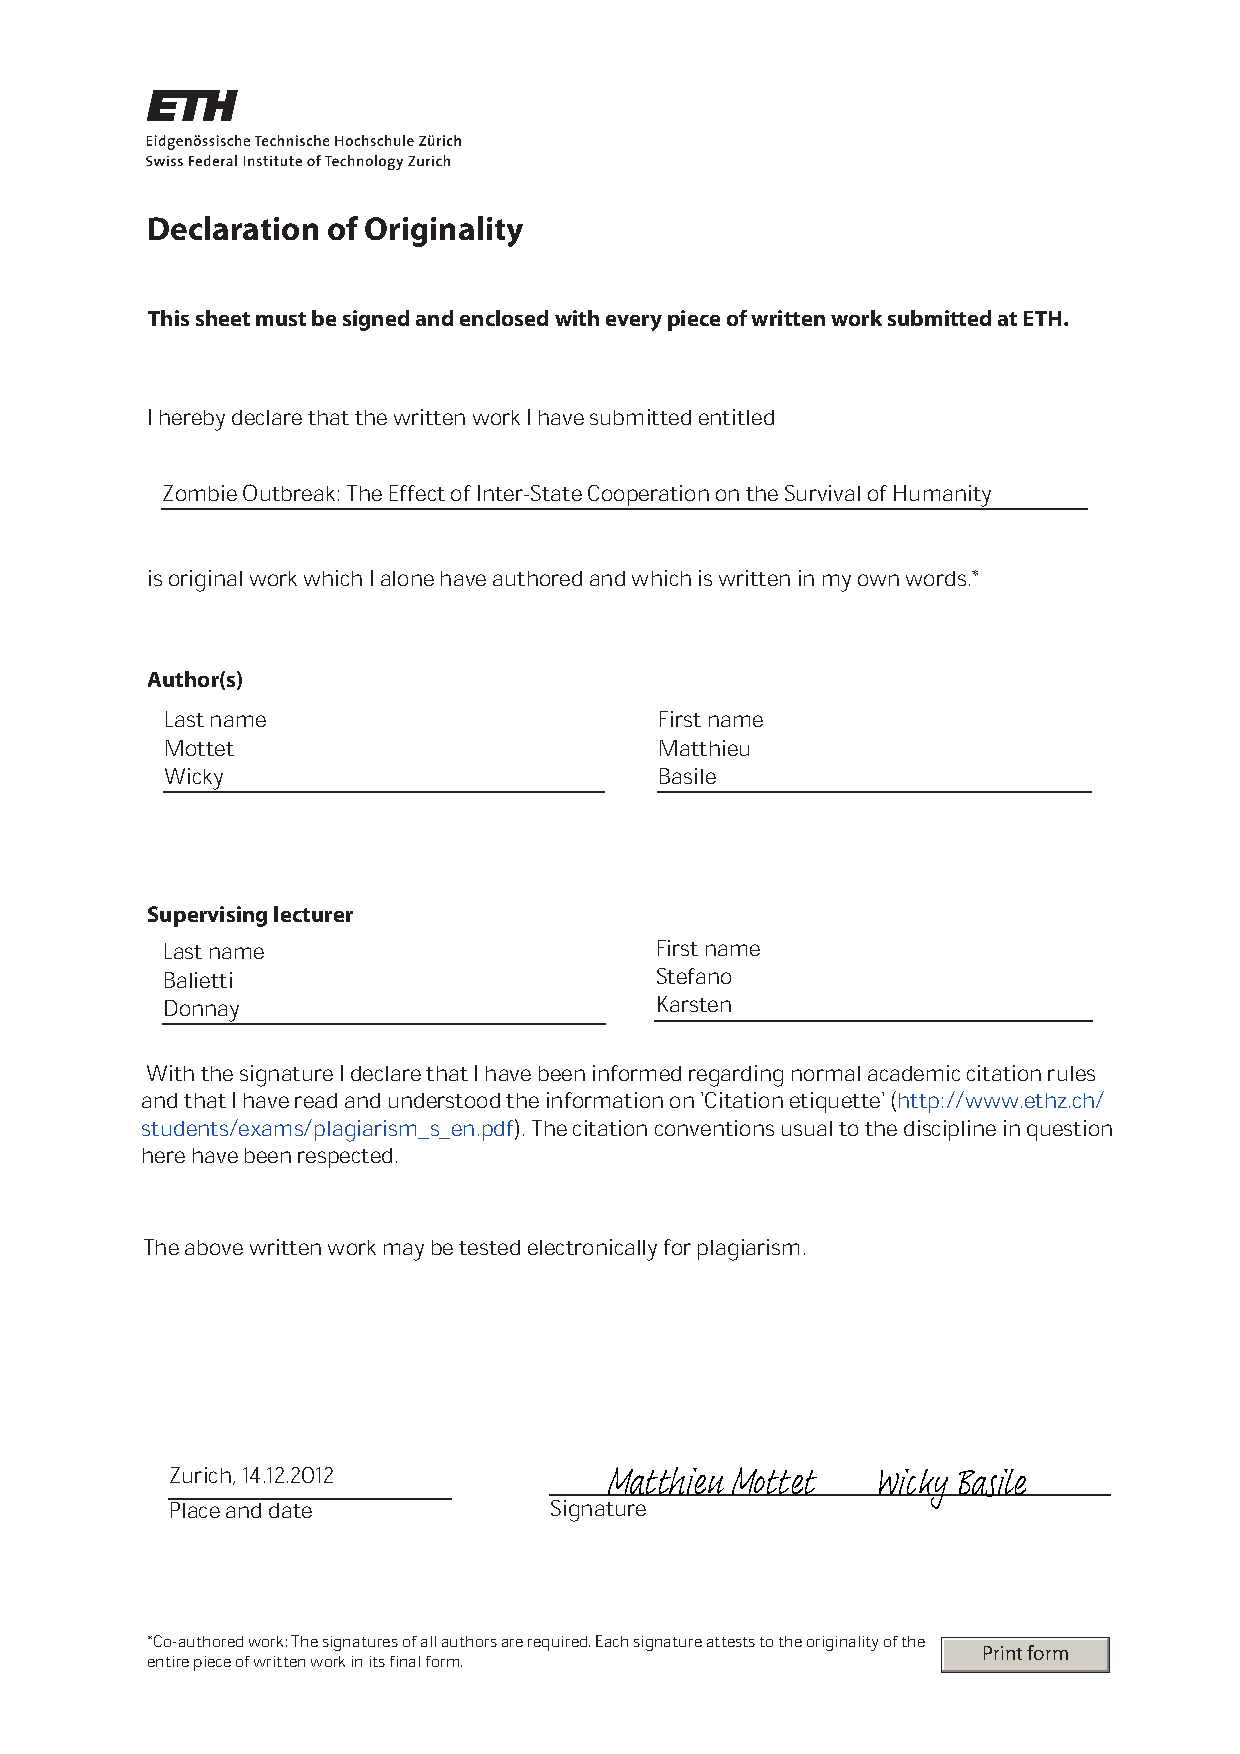
\includepdf{confirmation_en.pdf}

% TABLE OF CONTENT
\tableofcontents




% ABSTRACT 
\newpage

\section{Abstract}\indent

Application of an epidemiological model to a zombie outbreak has previously been investigated, raising the fear of dark days for humanity. Moreover, motivated by work in the field of international politics and the possible reactions of various foreign policies scenarios to such an event, we wished to deepen the investigation by expanding a SIR-like model to a multi-population system in order see how interactions between inter-connected populations may brighten the future of the human race. We developed a modification of the classical SZR model and added a framework to simulate inter-state transfers of populations. We then investigated the different regimes of our system through parameter variation. This analysis was made on two levels, first at the microstate (single state) then at the macrostate (international) level, in order to observe the influence of individual parameters on the simulation outcomes. We demonstrated that a system composed of intercating SZR model allowed to find regimes where humanity survived. However, a large dependence to the microstate parameters was noticed, whereas macrostate variables had a smaller impact These results suggest that the modelisation of the international population transfer might need to be re-defined.  


% INDIVIDUAL CONTRIBUTION
\section{Individual Contributions}\indent

M.G.M. and B.I.M.W. formulated the question in mathematical terms and discussed the implementation in MATLAB. M.G.M. wrote the code. M.G.M. and B.I.M.W. analysed and discussed the results and B.I.M.W. wrote the report.

% ACKNOWLEDGMENTS
\section{Acknowledgments}\indent

We wish to thank Karsten Donnay and Stefano Balietti for their support in our work, fruitful discussions and open-mindedness to accept such a project. We also would like to thank the Chair of Sociology for the computational support provided with simulation time on the ETH cluster Brutus.







% INTRODUCTION AND MOTIVATION
\newpage
\section{Introduction and Motivations}\indent

\subsection{Zombies: a Definition}\indent

The origin of the word ``zombie'' as well as its initial meaning is quite remote from modern popular culture descriptions. The word itself is said to have originated in the Carribean Voodoo spiritual belief system \cite{twohy2008voodoo, davis1997serpent}. During the ritual, a sorcerer would bring someone back from the dead and gain control on the reanimated corpse. The walking-dead no longer having a soul and being under the control of the voodoist, \textit{i.e.} lacking free-will, makes it a zombie. Some studies suggest that those ``zombified'' people were actually administrated a cocktail of natural drugs, one being tetrodoxin (a neurotoxin) as well as other hallucinogens \cite{davis1997serpent, littlewood1997clinical}. The toxin damages the brain, leading to apparent death and the vegetative state described as ``zombie'' in Voodoo beliefs.


Zombies in popular culture differ a lot from this anthropological definition. The canons of the zombie genre have numerous descriptions and hypothesis on both their characteristics and how they may have emerged in a human population. Since Romero's ``Night of the Living Dead'' \cite{nightofthelivingdead}, a turning point in the shift from Haitian folklore to modern depiction of reanimated-corpses, the r and origins of zombies have considerably evolved. More recent narratives usually describe the genesis of flesh-heating ghouls in an epidemiological sense, typically some sort of virus. Contemporary examples from the zombie genre include (non-exhaustively) ``Resident Evil'' \cite{residentevil}, ``28 Days Later'' \cite{28dayslater} and ``World War Z'' \cite{brooks2006world}. An outbreak stemming from Higgs radiation in a particle accelerator has recently been postulated as a possible source of flesh-eating monsters \cite{decay}. For simplicity, we will treat the cases of emergence and zombification as linked to an infectious disease of some sort, allowing the treatment of the problem using a modified epidemiological model. The main difference with a standard infectious disease where people get immunized is that being transformed into a zombie is a one-way process: the only way out is death.



\subsection{Zombie Outbreak and World Politics}\indent

Whilst international relations have already been studied under different pressure components \cite{gourevitch1978second, abrahms2013credibility}, the implications of a zombie outbreak on international cooperation has been underestimated and was almost never addressed. It is remarkable that the effect of such a dramatic event has not been looked at, although the fear of zombies and the threat they represent is vivid as reflected by the importance of the zombie genre in literature, films and videogames. Zombies, compared to other monsters such as vampires or aliens, have the very peculiar property not to be an exogenous species in the human population. Indeed they are still in a way human beings, simply somewhat altered, \textit{i.e.} zombified. Accordingly, zombies cause a much more deep-rooted fear as they not only threaten our lives by eating our brains, but also our sense of identity by questioning our notion of humanity. The psychological effects of such a non-standard threat, as well as the repercussions on the behavior of large population systems such as entire states, is likely to be significant. Accordingly, we decided to simulate an inter-state cooperation model in order to see the large-scale outcome of such an extreme event at an international level. While some people might question the validity of such a study, we believe that the applicability of such a reasoning could extend to other large-scale epidemiological disasters or simply give a line of reasoning to cope with what former U.S. Secretary of Defense Donald H. Rumsfeld referred as the ``unknown unknowns'' of international security \cite{seely2009pieces}. Zombies might not be real, but the threat and stress they could impose on world politics is.



\subsection{Popular Believes in the Event of a Zombie Outbreak}\indent

Epidemiological models have been well-studied to see the evolution dynamics and spread of diseases in populations \cite{brauer2008compartmental, riley2003transmission, Kuperman2001qy}. They are based on a model where interaction between susceptibles and infected, together with an infection constant, defines the rate of infection. In the simplest case, infected people can move to the immunized category following another mass-action law. These models have been shown to work in numerous cases and when corrections are added \cite{m1925applications, stone2007seasonal}, they can very well represent the evolution and spread of an infectious disease in a population. However, little investigations on epidemiological models with subpopulations have been performed.

It is interesting to realize that most zombie canons predict a very bleak outcome concerning the fate of humanity in the event of an outbreak. Indeed, most films and books describe an almost total extinction of humans and the few survivors are rarely in situations with foreseeable bright futures. While some might argue that the disappearance of the human race might not be such a regretful event and might actually benefit our planet \cite{paccalet2006humanite}, we wanted to see if the usual outcome for a zombie outbreak could differ from those classical scenarios, and if so, under which set of particular conditions. 

Mathematical modeling of a zombie outbreak in a single population has previously been investigated but showed very little hope for humans \cite{munz2009zombies}. The primary reason for the annihilation of humanity in all of the presented scenarios lies in the models simulated by the authors. In contrast to classical epidemiological models where infected people can recover by going from susceptible to removed in a immunized sense of the term, the zombie scenario differs quite a bit. Now ``removed'' is no longer synonym of ``immunized''; it is actually a gentle way of describing death. Accordingly, under the considerations of the authors' model, humans can only die and this eventually occurs in every case.



\subsection{How Could Humanity Survive?}\indent


We rationalized that a state-based description of the world, with subpopulations, might not only be more realistic for the modeling of a global scale zombie outbreak, but might actually help brightening the outcome in such an occurrence. The world is divided into states that apply their own laws and restrictions in terms of immigration. If immigration applies to humans, it might as well apply to zombies. In such a case, one might envision that, in a given state under a zombie epidemiological threat, fluxes of incoming humans to help kill zombies or emigration of survivors to non-infected states might lead to brighter outcomes that the classical end-of-the-world scenario. It would also be imaginable to observe the emergence of a zombie state while all the remaining survivors would have found shelter elsewhere; or that the help of susceptibles from another state might help eradicate the new zombie threat. 

We decided to simulate a model of interacting subpopulations, each under an epidemiological treatment of the zombie infection. The inner-state model describes the emergence of zombies from a spreading disease point of view, while the population fluxes between states would represent migration of populations. 

Moreover, we were interested in seeing to what extent the different paradigms of international politics, \textit{Realpolitik}, Liberalism and Neoconservatism, as defined by Daniel W. Drezner in \textit{Theories of International Politics and Zombies} \cite{drezner} may lead to different outcomes if taken into account in our model. 

% DESCRIPTION OF THE MODEL
\newpage
\section{Description of the Model}\indent

In order to simulate a multi-state system under epidemiological evolution, we needed to define a clear mathematical framework treating both the population transfers within states and among states. Such a treatment was necessary to represent the twofold representation of a zombie outbreak at an international level composed of well-defined states:
\begin{enumerate}[i.]
	\item Intra-state fluxes represent the true epidemiological part of our model. They have a fixed physical definition and are mostly invariable among states.
	\item Inter-state fluxes do not represent epidemiological variation \textit{per se} but a modeling of migration fluxes. They will depend on the paradigm of international politics under consideration. 
\end{enumerate}

With such an approach, we should be able to evaluate the population evolutions at the international and domestic levels. The idea would be to see if variations of international fluxes could influence the global outcome in terms of survival of our species. Moreover, we were interested in the modalities of such a survival. Would the zombies be eradicated? Would some states disappear? Is the emergence of a zombie state possible? Of course, owing to the complexity of a world-scale epidemics involving zombies, we had to make some basic assumptions in order to formulate a mathematical treatment of the system, namely:
\begin{enumerate}[i.]
	\item Zombification is infectiously transmitted upon contact between susceptibles and a zombies.
	\item Zombification occurs instantaneously without latent infectious phase.
	\item The outbreak occurs over a short amount of time. Therefore, both natural death rate and birth rate can be neglected.
	\item Only three types of homogenous populations are considered, susceptible (S), zombie (Z) and removed (R).
\end{enumerate}

We chose to simulate the microstate level under a modification of the classical SIR model called the SZR model (S for Susceptibles, Z for Zombies, R for Removed) \cite{munz2009zombies}. In contrast to the original SZR model developed by the authors, we made two modification in order to accommodate our interpretation of the epidemiology of zombies. As we could not find an appropriate treatment of an epidemiological model with distinct subpopulations that would fit a zombie outbreak, we had to develop a treatment for the macrostate population transfers that would fit our description of international cooperation in such a scenario. Since removed represent dead humans or head-shot zombies, they cannot transfer between states and accordingly only the transfer of S and Z needs to be considered. 

\subsection{Microstate Description}\indent
\label{sec:microdescription}

Each state (microstate) has three distinct populations, the susceptibles (S), the zombies (Z) and the removed (R). They define the components the SZR model. A scheme for the microstate fluxes is described in figure \ref{microstate}.

% Microstate model figure
\begin{figure}[h!]
\centerline{
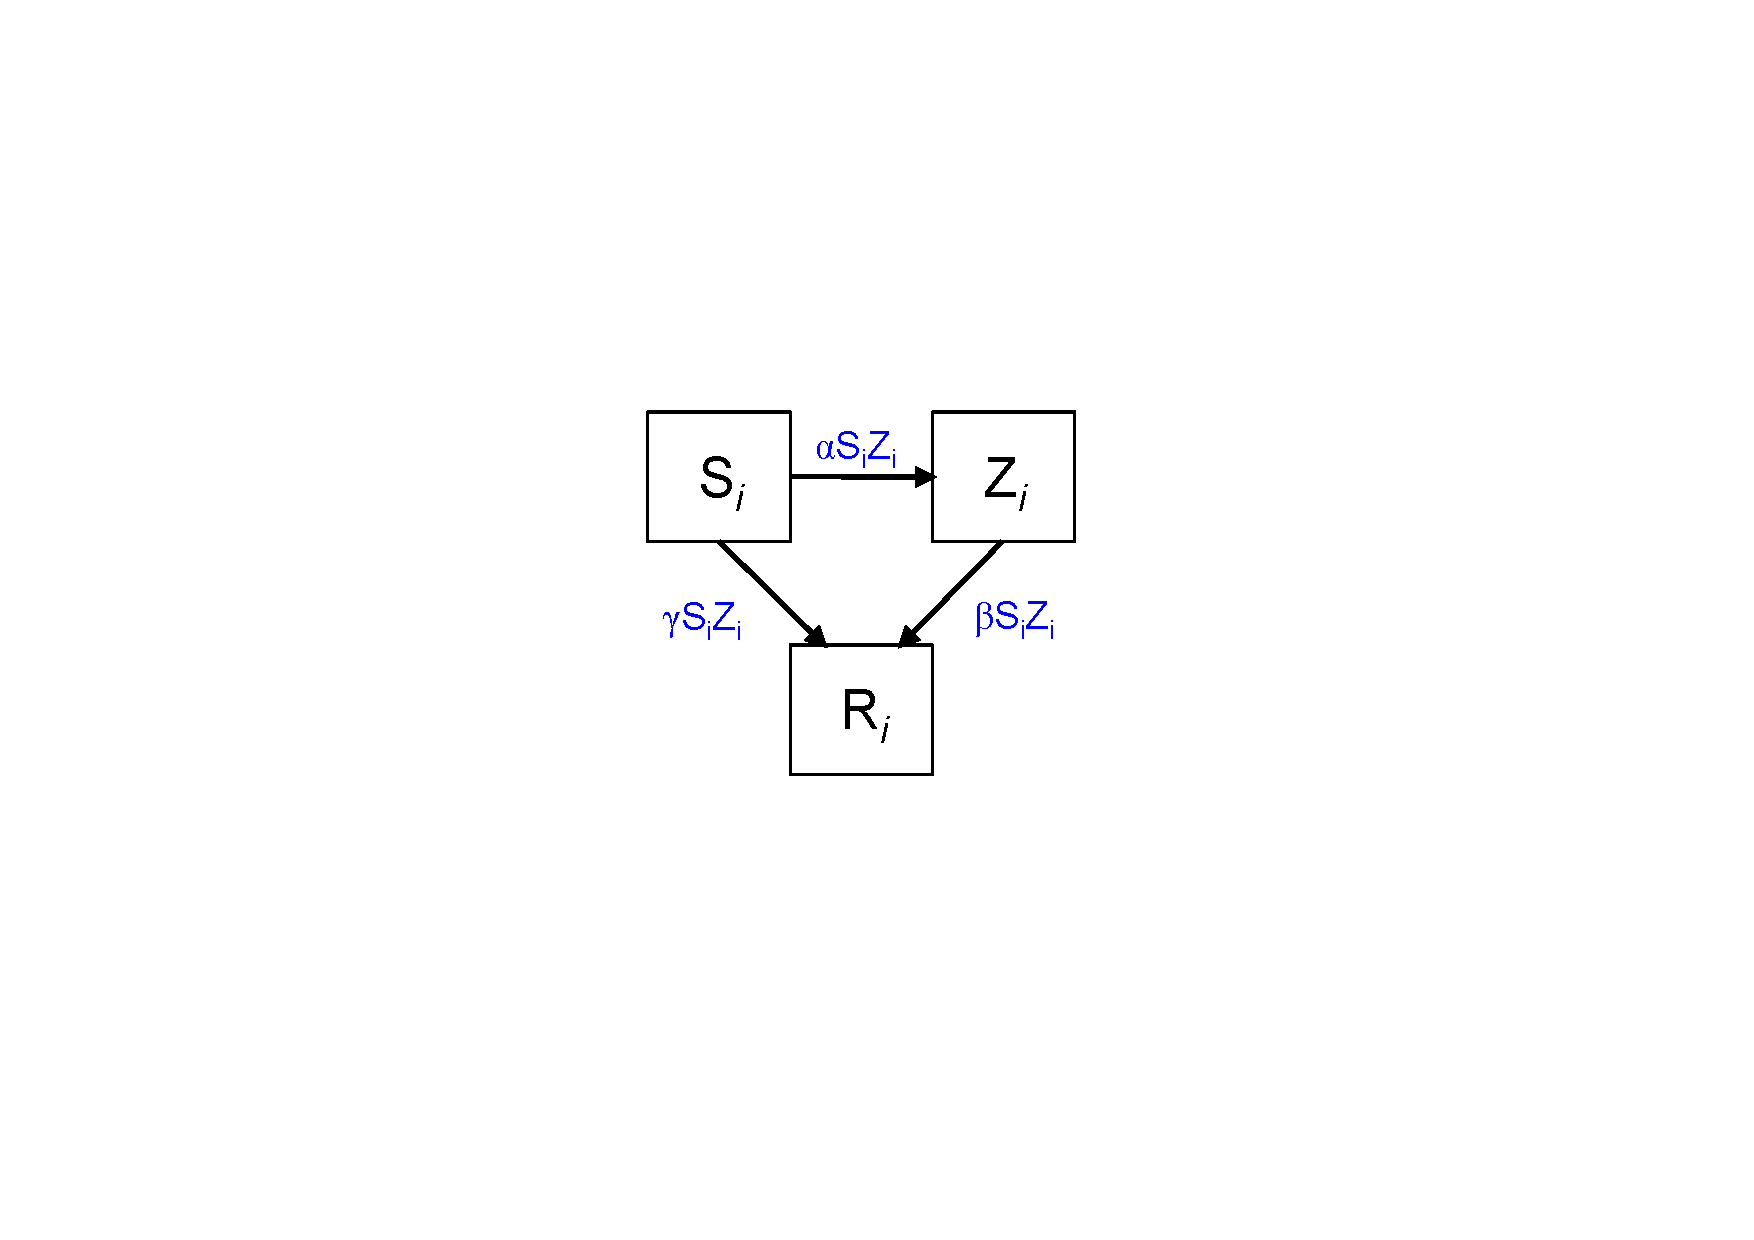
\includegraphics[scale=0.55]{../images/Powerpoint_figures/microstate.pdf}}
\caption{Description of population fluxes at the microstate level. \label{microstate} }
\end{figure}

Unlike the original SZR model described by Munz \textit{et al.} \cite{munz2009zombies}, we do not consider dead rising from their graves to become zombies as it allows an endless regeneration of the zombie population through the sequence $Z\rightarrow R\rightarrow Z$. In contrast, we consider a more modern approach to the zombie type as described in recent works of the genre. It includes considerations such as removal of the head effectively killing a zombie and the impossibility of \textit{post mortem} infection. As such, the source for new zombies can only be from susceptibles.  Moreover, we consider that non-natural death of susceptibles directly to the removed population is a mass-action transfer of both the zombie and susceptible populations multiplied by a constant $\gamma$. The rationale behind formulating the fluxes as such comes from the interpretation that those deaths are zombie-related, such as forced escapes, crowd panic and other consequences of large-scale disasters. Furthermore, susceptibles become zombies through the same mass-action equation, where the rate of infection is $\alpha$. Taken together, these elements give equation \eqref{eq:smicro} for the variation of the susceptible population. The zombie population has an incoming flux from the susceptible with parameter $\alpha$ as previously described. They can also get killed through encounters with susceptibles with a frequency proportional to the rate constant $\beta$. Taken together, these two equations describe the flux of zombies at the microstate level \eqref{eq:zmicro}. From those mathematical relationships logically come the description of the removed variation (equation \eqref{eq:rmicro}). 

\begin{equation}  \label{eq:smicro}
\Delta S_{i}^{micro} = -\alpha S_{i} Z_{i} -\gamma S_{i} Z_{i} = -(\alpha + \gamma) S_{i} Z_{i}
\end{equation}

\begin{equation} \label{eq:zmicro}
\Delta Z_{i}^{micro} = +\alpha S_{i} Z_{i} - \beta S_{i} Z_{i} = (\alpha - \beta) S_{i} Z_{i}
\end{equation}

\begin{equation} \label{eq:rmicro}
\Delta R_{i}^{micro} = +\beta S_{i} Z_{i} + \gamma S_{i} Z_{i} = (\beta + \gamma) S_{i} Z_{i}
\end{equation}
\bigskip

It is noteworthy to already mention that under such a treatment, which considers an outbreak occurring over a short amount of time, the population of susceptibles can only decrease (two outgoing fluxes, no incoming flux) and the population of removed solely increase (two incoming fluxes, none outgoing) no matter what the choice of parameters is. The variation of the zombie population can, however, be either positive or negative, depending on the ratio between $\alpha$ and $\beta$. Another interesting feature of this model is the identical mass-action description of all the fluxes (proportionality to $S_{i} \cdot Z_{i}$), meaning that the outcome will be solely dependent on the ratios between the parameters $\alpha, \beta$ and $\gamma$.

\subsection{Macrostate Description}\indent

Whilst description of the microstate was fairly obvious from literature precedents, a simple description of population transfers at the macrostate proved to be challenging. Indeed, it had to describe the complexity of population migration at the international level in the context of a large-scale epidemiological disaster. It also had to capture and describe the behavior of a so far unknown actor on the international scene; namely zombies. The baseline migration of susceptibles (in the absence of a zombie outbreak) was supposed to be negligible in comparison to population exodus from zombie fear and accordingly not modelled in our transfer description. We initially wanted to implement another mass-action transfer of susceptibles related to the respective ratios between S and Z in the different populations (susceptibles would not migrate to a state where humans would already be overwhelmed). However, this description might not be realistic as it implies knowledge of the infection status of the state to be migrated in; an unlikely fact in a scheme of panic migration. Moreover, this model proved to be very hard to implement for convergence and update criteria due to the high inter-dependence of the multiple subpopulations. It was therefore replaced by another model described by equation \eqref{eq:smacro}. 

\bigskip
\begin{equation} \label{eq:smacro}
\Delta S_{i}^{macro} =  \sum_{j\neq i}{ \left( \nu \langle \Delta S_{j} \rangle - \nu  \langle \Delta S_{i} \rangle \right) }
\end{equation}
\bigskip

In this description, susceptibles emigrate symmetrically to all the other states, irrespective of their infection status (ignorance model). Emigration pressure is generated by calculating the mean of the last ten variations of susceptibles in the state. The justification for such a treatment of the migration is that if a large number of susceptible deaths and zombification occurred over the recent updates, the remaining population would be more inclined to move away from the ``disaster'' zone (panic model). Besides, the use of a sliding window to calculate the mean fluctuation introduces a latent effect on the emigration, consistent with large crowd displacement in a moment of panic. 

% Macrostate model figure
\begin{figure}[h!]
\centerline{
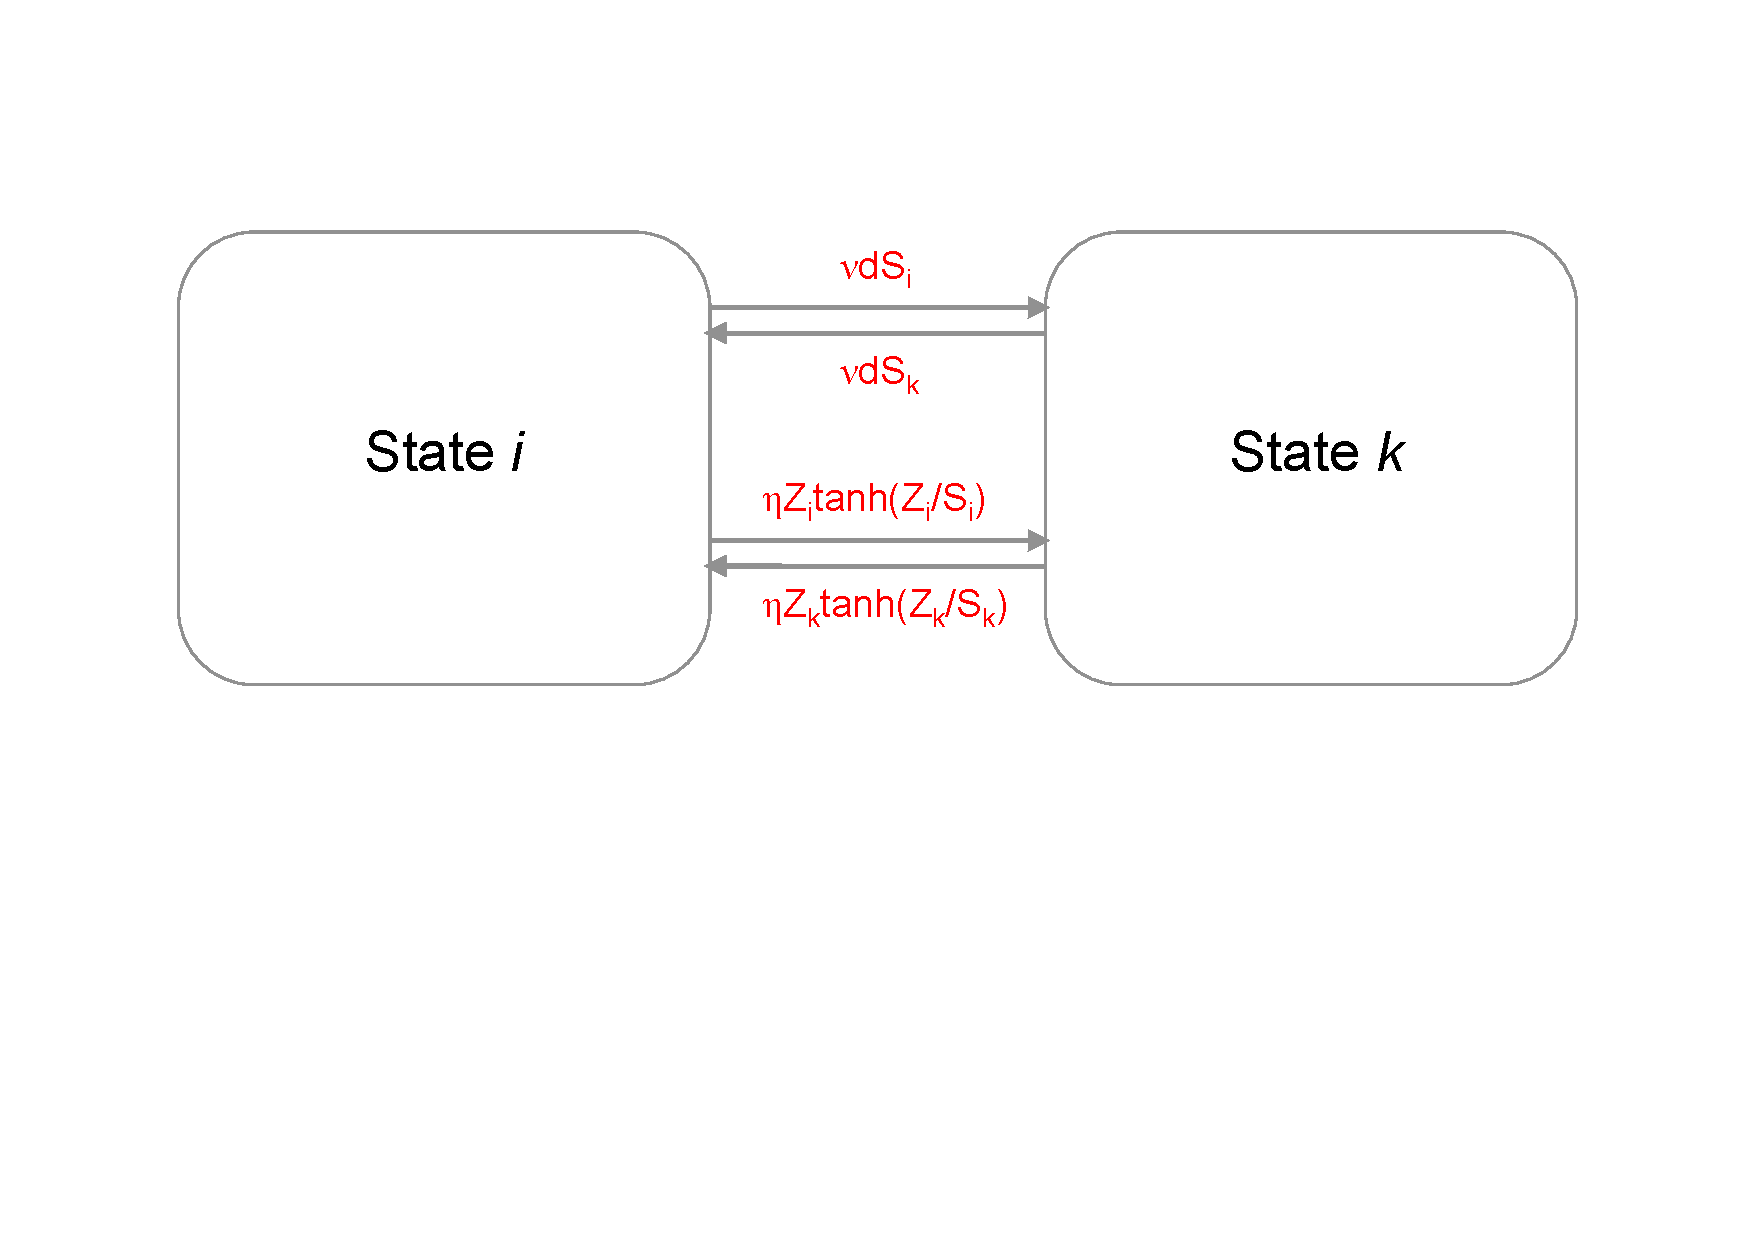
\includegraphics[scale=0.40]{../images/Powerpoint_figures/macrostate.pdf}}
\caption{Description of population fluxes at the macrostate level.
\label{macrostate} }
\end{figure}


Description of the zombie migration was more problematic owing to the lack of unambiguous zombie behavior in the literature. Two descriptions of behavioral types for zombies is usually found. It is usually either in the framework of a random-walker, \textit{i.e.} its pattern of motion is completely independent of its surrounding, or it is based on a flesh-craving interpretation, \textit{i.e.} zombies will go where humans can be found. Our initial try was to study a flesh-craving type of zombie. However, the implementation failed for the same reasons as the initial susceptible migration model, namely the need for a mass-action description generating too large of a dependence between all the subpopulations and an impossibility to generate the population update. We then decided to revise our description of the type of zombie considered in order to reduce the dependence of the calculation to the different populations. We described a pseudo-flesh-craving zombie where emigration pressure to another state is dictated by the ratio Z over S in the state from which it emigrates. In other terms, the little availability of ``local'' food would push the zombies to look for new horizons. In this description, the knowledge of the other state's statues is unknown to the zombies, which is probably of fair representation of reality since zombies are not intelligent species and cannot get information through \textit{e.g.} news channel. Equation \eqref{eq:zmacro} gives the mathematical description of the zombie flux at the macrostate level. 

\bigskip
\begin{equation} \label{eq:zmacro}
\Delta Z_{i}^{macro} = \sum_{j\neq i}{\left( \eta Z_{j}\tanh \left( \frac{Z_{j}}{S_{j}}\right) -\eta Z_{i}\tanh \left( \frac{Z_{i}}{S_{i}}\right) \right)}
\end{equation}
\bigskip

The use of $\tanh$ for the ratio was implemented in order to avoid infinite emigration of zombies when the population of susceptible tends to zero, which would generate unphysical results. Since $\tanh$ can only take values between 0 and 1, we multiplied the equation by the actual zombie population, making the emigration proportional to the current number of flesh-eating ghouls. Figure \ref{macrostate} describes the relationship between two states, \textit{i} and \textit{k}.





\subsection{Model with Three Interconnected States}\indent

We decided to simulate the evolution of a zombie population (initially sparkled in a single state) for a system of three interconnected states and see how the choice of parameters, in particular $\nu$ and $\eta$ (international cooperation factors), might affect the outcome on the global scale. Figure \ref{totalmodel} gives a representation of the model we implemented. We initially wanted to make those macrostate parameters time-evolving under a game-theoretical treatment, unfortunately, time-limitation made this implementation impossible (see \ref{sec:gt} for details about such a treatment).
 
% Total model figure
\begin{figure}[h!]
\centerline{
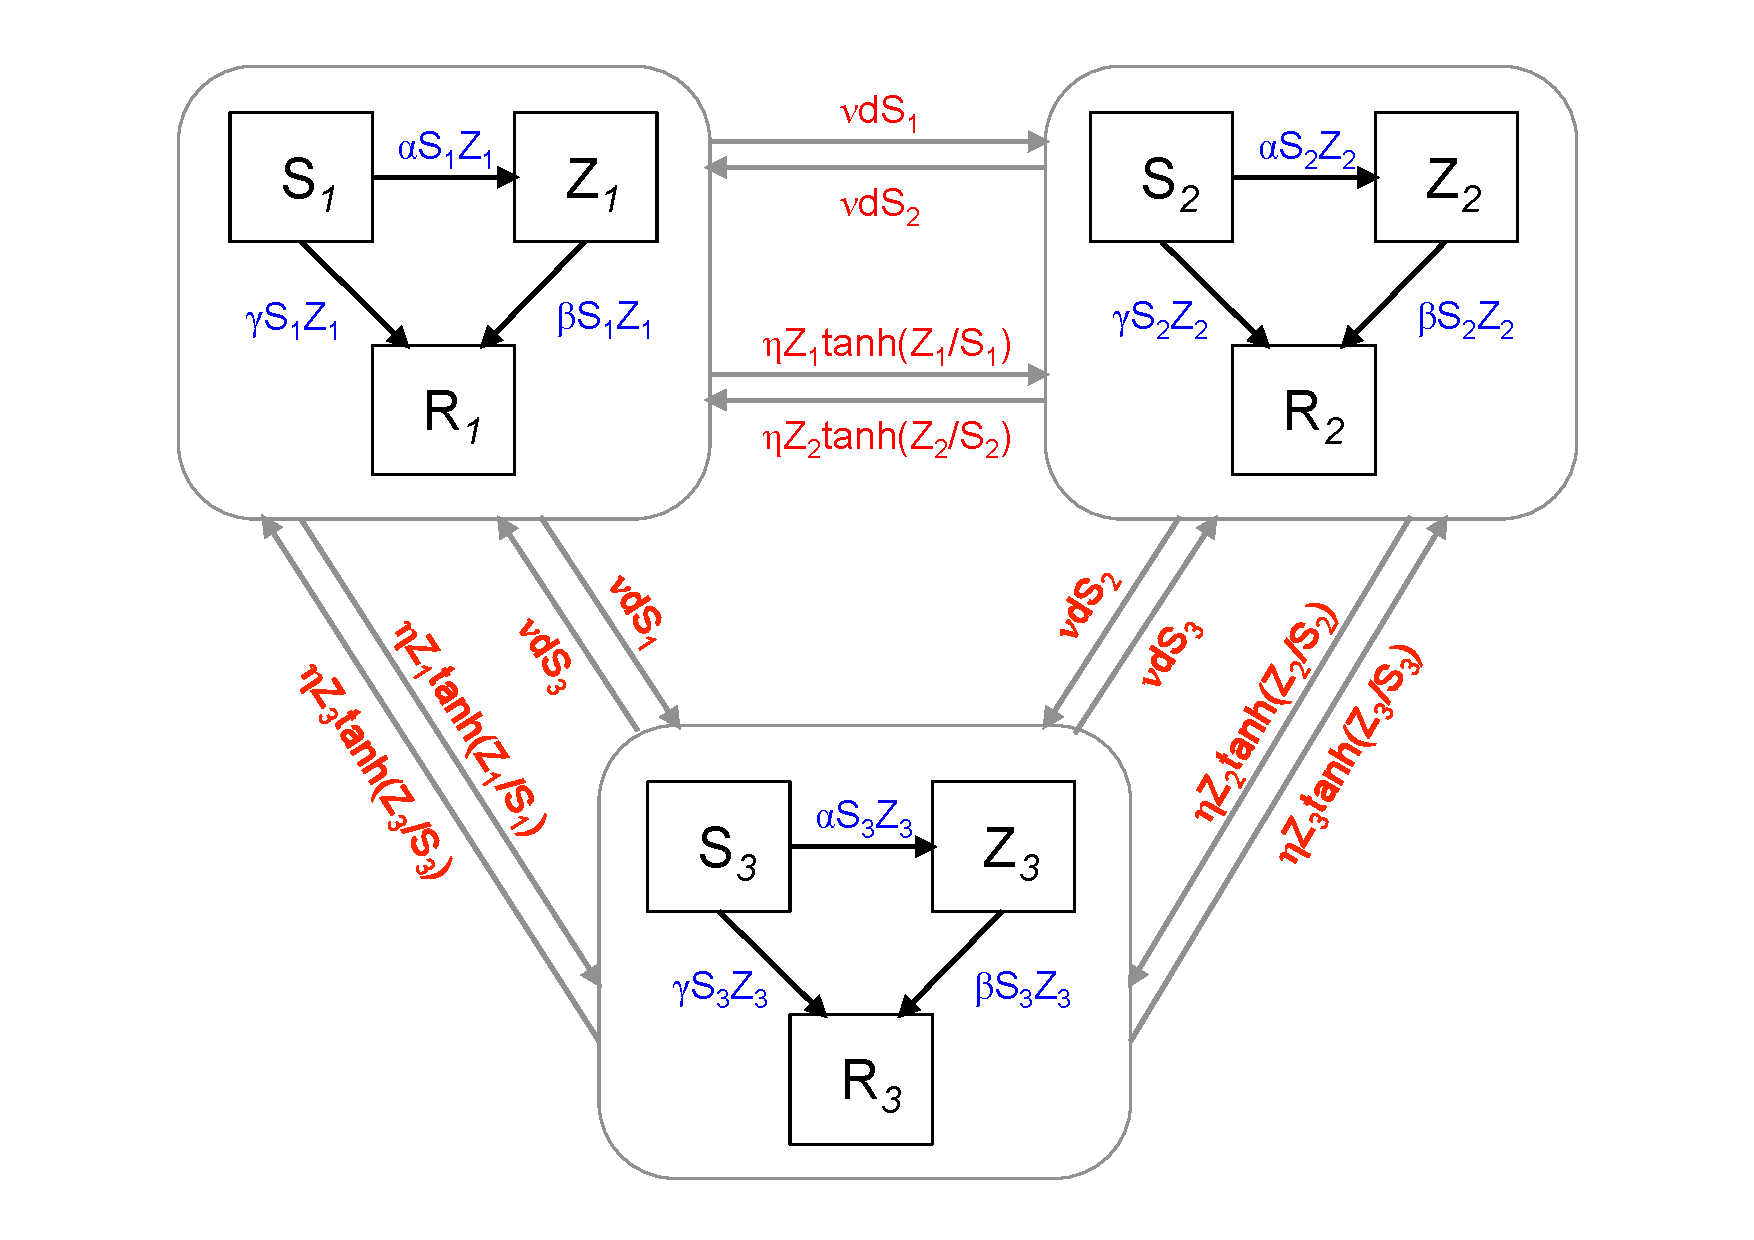
\includegraphics[scale=0.43]{../images/Powerpoint_figures/total_model.pdf}}
\caption{Schematic representation of our 3-state model including all variables and fluxes. The parts in blue represent the fluxes between the population S, Z and R at the microstate level while the parts in red represent the macrostate fluxes of S and Z.\label{totalmodel} }
\end{figure}


Due to the high inter-dependence of all the parameters, it was difficult to deconvolute the effect of each on the outcome of the individual simulations. Since quantitative data that would have allowed the generation of parameters for zombification ($\alpha$), zombie-killing ($\beta$) and death related to zombies ($\gamma$) were absent from the literature, it was necessary to determine them by parameter sweeping. Once interesting regimes and phase transitions for $\alpha, \beta$ and $\gamma$ were found, investigation of the effect of $\nu$ and $\eta$ were performed.


% IMPLEMENTATION
\newpage
\section{Implementation}\indent

The implementation in MATLAB works on two levels: the first is responsible for the management of the simulation while the second is taking care of the stepwise update of the simulation. We will discuss the key parts of the implementation as well as some of the special features used to ensure the coherence and convergence of the simulations. Moreover we will discuss some additional functions used for the sweeping and analysis of the results.


\subsection{The Outbreak Function}\indent
\label{outbreakimpl}

The outbreak function is the wrapping function of the epidemiological model. It first evaluates the different parameters, initializes the different matrices used throughout the simulation, calls the update function and finally validates the new data generated after each update cycle. The validation of the data tests if it is worth continuing the simulation or if it should be terminated to save computational time. We implemented three exit policies in the simulation loop. First, we implemented two obvious safeguards when either the susceptible or the zombie population reaches zero. Continuing the simulation in either case would not make sense since the system already reached its final state. The third one is triggered when the different population evolutions become too slow, indicating a pseudo steady-state. Even though it might not be a true dynamical equilibrium, little population variation over a very long time would not be of any significance within the framework of our model (\textit{e.g.} a single zombie slowly killing thousands of remaining humans over the course of a very long simulation). In order to avoid this unphysical result, we defined the following control:

\bigskip
\begin{equation} \label{eq:outbreakequilibrium}
\left\langle \left| \Delta S \right| \right\rangle < x\ \&\&\ \left\langle\left|\Delta Z \right| \right\rangle < x
\end{equation}
\bigskip

Where $x$ is the threshold value. The mean of the absolute variation of susceptibles and zombies is calculated for the last 100 steps using a sliding window and compared to a threshold $x = 0.1$. If the values are smaller than the threshold, we assume a steady-state or ``quasi-equilibrium'' and the simulation is terminated. Furthermore, a maximum number of step can be defined (default: $10^8$ steps) as last exit condition (see \ref{sec:outbreak} for details about the code).

\subsection{The Update Function}\indent

The update function takes care of the evolution of the different populations at each cycle. It applies the different equations of our model (see equations \eqref{eq:smicro}, \eqref{eq:zmicro}, \eqref{eq:rmicro}, \eqref{eq:smacro} and \eqref{eq:zmacro}) and uses safeguards to ensure generation of physically meaningful results. It first calculates the variation-to-be of the susceptible populations based on the current populations and executes the different control procedures. Once the susceptible populations are updated, the zombie population is considered in a similar manner, except for the S to Z fluxes, where the previously obtained values are used. The control procedures are done in order to ensure that negative populations do not arise. Finally, the removed are obtained using the fluxes previously calculated.

The first constraint is applied during the computation of the flux exiting each state. Due to the structure of the program, negative population values can arise. Although these values will be extremely small ($> - 10^{-4}$), resulting in small positive exiting fluxes, they will lead to negative entering fluxes in the other states. These fluxes being considered as positive in the next control procedure, negative values have to be avoided.

The second constraint is applied after the computation of all the fluxes. There is the possibility for the negative fluxes (death, contamination and emigration) to be larger than the population before update plus the incoming flux (immigration). In such cases, we apply an algorithm to avoid apparition of negative populations. According to equations \eqref{eq:smicro} and \eqref{eq:smacro}, the total variation of susceptibles in state \textit{i} is defined by four negative fluxes and two positive ones.

\bigskip
\begin{equation} \label{eq:delta-}
\Delta S_i^- = \Delta S_{S\rightarrow Z} + \Delta S_{S\rightarrow R} + \Delta S_{S_i\rightarrow S_{j\neq i}} + \Delta S_{S_i\rightarrow S_{k\neq i}}
\end{equation}

\begin{equation} \label{eq:delta+}
\Delta S_i^+ = \Delta S_{S_{j\neq i}\rightarrow S_i} + \Delta S_{S_{k\neq i}\rightarrow S_i}
\end{equation}
\bigskip

For the value of the population to stay positive, the following relation has to be true:

\bigskip
\begin{equation} \label{eq:condition}
S_i + \Delta S_i^{tot} = S_i + \Delta S_i^+ + \Delta S_i^- \geq 0
\end{equation}
\bigskip

If this condition is not fulfilled by every state, the fluxes are redefined according to equation \eqref{eq:correction} in order for the relation to be true and the ratios between the different negative fluxes to remain unchanged compared to the initial ones:

\bigskip
\begin{equation} \label{eq:correction}
\Delta S_{X\rightarrow Y,1} = \frac{\Delta S_{X\rightarrow Y,0}}{\Delta S_i^-}\cdot max(\Delta S_i^+ + S_i, 0)
\end{equation}
\bigskip

After the update of the four negative fluxes, the corresponding inter-state variations are updated. This procedure is repeated until all states fulfill the condition. Note that a convergence criterion has been defined to account for computational numeric inaccuracies. This criterion allowing minor negative values (up to $10^{-4}$) for the resulting populations, zeroing of the negative values of $S_i + \Delta S_i^+$ is essential to avoid inversion of the fluxes in \eqref{eq:correction}. A similar procedure based on equations \eqref{eq:zmicro} and \eqref{eq:zmacro} is applied to the zombie population. This safeguard method allows a relatively fast convergence in the calculation of the corrections while retaining physical significance for the corrected values (see \ref{sec:update} for details about the code).



\subsection{The Sweep Function}\indent

The sweep function acts as a tool for the automatized sweeping of each parameters between two values using defined steps. The results of each individual simulation are stored in a dedicated folder. It also assigns an identification string to the sweep, allowing to resume from the last completed simulation. This feature was added in order to be able to interrupt long simulations performed on personal computers and resume them later (see \ref{sec:sweep} for details about the code).


\subsection{The FindTransition Function}\indent
\label{sec:findTransition}

In order to analyze our multidimensional sweeping, we implemented a function to find the transition between three parameters allowing the survival of the humanity and those leading to its doom. The function recovers the coordinates of all points whose value is not zero in a 3D matrix and for each, controls if one of the six neighbors has a value equal to zero. If this is the case, the original value is returned, otherwise the point is zeroed. This allows to visualize the phase transition in the $4^{th}$ dimension (see \ref{sec:findtrans} for details about the code).





% SIMULATION RESULTS AND DISCUSSION
\newpage
\section{Simulation Results and Discussion}\indent

Due to the high interconnectivity of our model and the dependence of every parameter towards each other with respect to simulation outcome, we decided to first split the components of our model to observe their behaviors independently and be able to deconvolute the role of the different population fluxes on the overall outcome scenario. The first obvious treatment was to look for the different regimes of our SZR model in the isolated case (no connection to other states). Secondly, we wanted to look for the different regimes accessible when we connected three states to form our full model. Obviously, full understanding of the role of each of the five parameter when treating the international case required parameter sweeping in order to treat each effect separately. Unfortunately, due to the number of parameters present in our model (five), full parameter sweep and analysis would have required plotting in the $6^{th}$ dimension. In addition, the number of individual simulation would have been enormous and impossible to analyze. Although imperfect, we decided to separate the parameter sweep of the micro- and macro-state levels. We rationalized that we could first sweep $\alpha$, $\beta$ and $\gamma$  to find the interesting phase transitions at the microstate level and then take some $[\alpha, \beta, \gamma]$ triplet to sweep parameters $\nu$ and $\eta$ and observe the interesting regimes at the international level. This allowed us to make suppositions regarding the type of foreign policies that should be adopted to maximize the chances of survival of the human race in the event of a zombie outbreak. 

\subsection{Population Time-Evolution in an Isolated State}\indent
\label{szr}

Although a similar model had previously been studied \cite{munz2009zombies}, we wanted to investigate the behavior of our modified SZR model (under isolation), in particular the potentially different types of regimes accessible in contrast to the ever-fatal outcome of the original SZR model. As previously discussed (see \ref{sec:microdescription}), all transfers at the microstate level follow the same mass-action law and accordingly different outcome will depend solely on the various ratios between the parameters of the SZR model ($\alpha$, $\beta$ and  $\gamma$). We can already predict, in the case of an isolated state, that the variation of S will always be negative and variation of R will always be positive. Variation of Z will depend on the $\alpha/\beta$ ratio. Figure \ref{deathS} shows the time-evolution of the different populations (S, Z, R) when contamination is started by a single zombie for the cases $\alpha>\beta$ and $\alpha=\beta$.
% Susceptible always dead (independent of gamma)
\begin{figure}[h!]
\centerline{
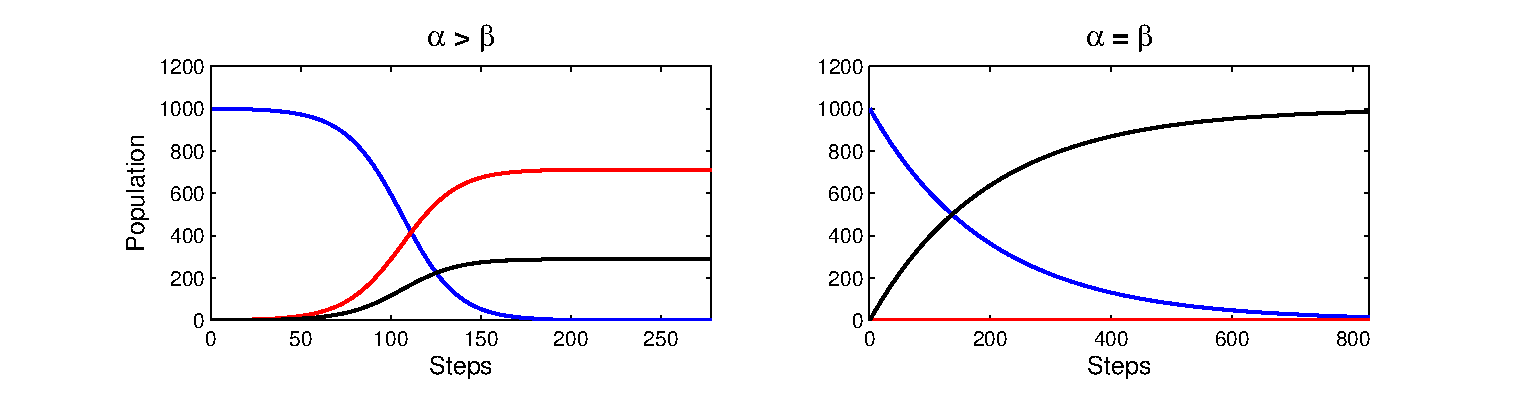
\includegraphics[scale=0.65]{../images/Matlab_figures/model-AgeB.eps}}
\caption{Doomsday scenarios for an isolated state. Left: outbreak of zombies due to an unfavorable $\alpha/\beta$ ratio. Right: extinction of the human race with no zombie outbreak. In that limiting case, humans turn into zombies as fast as zombies get killed, but zombie-related deaths alone are sufficient to eventually lead to annihilation of the all humans (\textcolor{blue}{blue} = susceptibles, \textcolor{red}{red} = zombies, black = removed. Left: $\alpha=1.6\cdot10^{-4}, \beta=1.0\cdot10^{-4}, \gamma=8.0\cdot10^{-5}$. Right: $\alpha=5.0\cdot10^{-3}, \beta=5.0\cdot10^{-3}, \gamma=8.0\cdot10^{-5} $). \label{deathS} }
\end{figure}

It is worthwhile noting that the doomsday scenario observed in both cases occurs irrespectively of the value of $\gamma$. The only effect of $\gamma$ is on the speed at which the human race gets wiped out from the surface of the earth. This understandable since in both cases ($\alpha\leq\beta$) apparition of zombies occur at a rate greater or equal than they get killed and therefore they will eventually overcome our planet. The parameter $\gamma$ (representing zombie-related death but not zombification) is only an additional way humans die but does not affect the zombie population directly. Another interesting observation one can make from figure \ref{deathS} is the difference in regimes when $\alpha<\beta$ and $\alpha=\beta$. In the first case, we see a classical doomsday scenario where the zombie outbreak gradually leads to the disappearance of all humans with a few ``collateral'' damages as well. The second scenario presents an interesting feature. Indeed, no real zombie outbreak occurs (since we start with one zombie and the rate of zombification is equal to the rate of extermination) but humans still disappears, triggered by the zombie-related deaths. This could be rationalized for a situation where a small zombie niche would exist and humans would try over and over again to kill them but with each attack-wave, the number of infected would equal to the number of killed and other humans would be killed in the process as well. Finally, it is worth seeing that these two regimes would be similar if a greater initial number of zombies was present, with the only difference that convergence would be reached faster. 

Those two regimes represent the death of humanity. What would the parameters need to be in order to see the survival of the human race and what would they represent in real-life terms? From the relationship between the SZR parameters previously described, it is obvious that for humans to survive in any case, the combined rates of their disappearance needs to be smaller than that of the killing of zombies ($\alpha+\gamma<\beta$). In the case where $\alpha<\beta$ (zombification is slower than the destruction of zombies) but  $\alpha+\gamma>\beta$ (overall, humans still die at a greater rate due to the zombie-related deaths), the initial number of zombie matters in terms of outcome and survival of humanity. Those two regimes are shown in figure \ref{gamma_population}.



% dependence to gamma and population
\begin{figure}[h!]
\centerline{
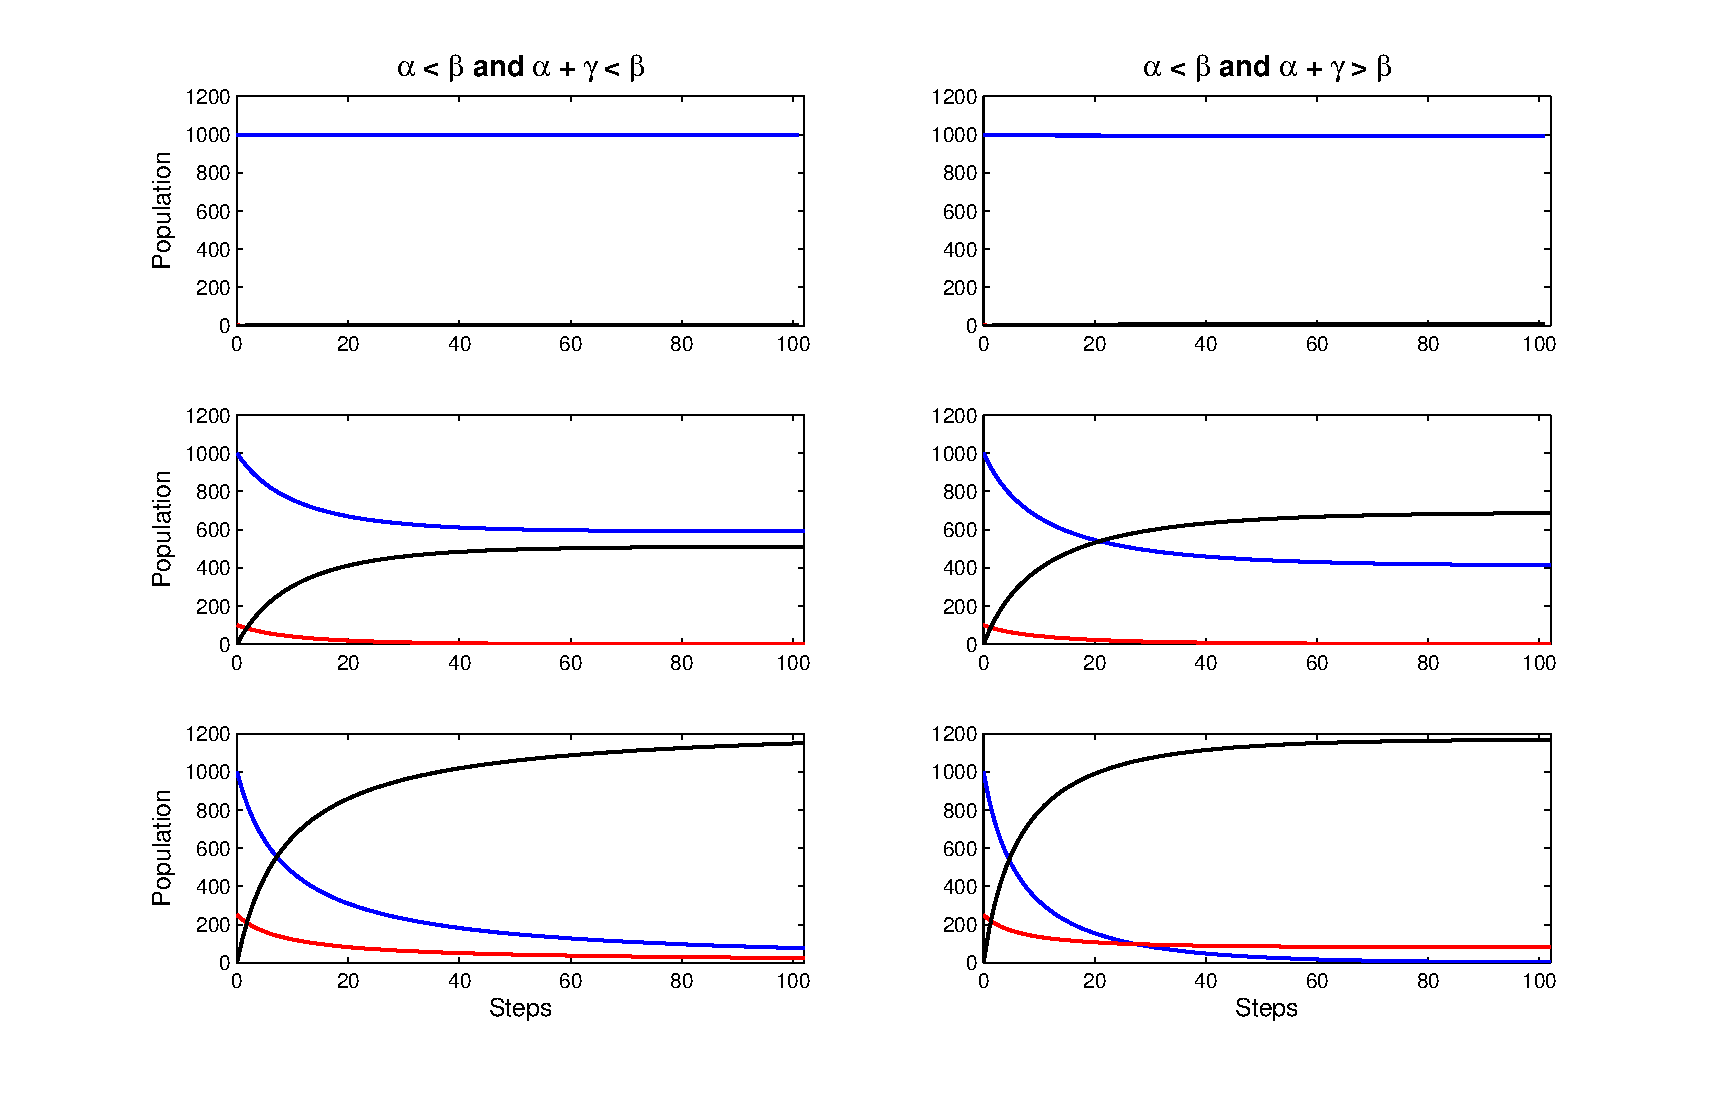
\includegraphics[scale=0.55]{../images/Matlab_figures/model-AltB.eps}}
\caption{The effect of $\gamma$ in the limiting case $\alpha<\beta$. In this particular scenario, the weight of $\gamma$ shifts the overall disappearance of susceptibles compared that of zombies from smaller (left) to larger (right). The initial number of zombies will affect the outcome in the latter case but will not jeopardize the survival of humanity in the former case. (\textcolor{blue}{blue} = susceptibles, \textcolor{red}{red} = zombies, black = removed. $\alpha=4.0\cdot10^{-4}, \beta=5.0\cdot10^{-4}$ for all simulations. Left column: $\gamma=0.1\cdot10^{-4}$, right column: $\gamma=1.9\cdot10^{-4}$. Initial number of zombies: first line=1, second line=100, third line=200). \label{gamma_population} }
\end{figure}

It is observable that with a starting number of one or a hundred zombies, humanity survives in both cases. However, we can see that when the starting number of zombies is two hundreds, then the scenarios diverge. The situation where the overall death of humans is greater than the death of zombies (right column) leads to extinction of humanity because the combined ``collateral'' deaths and zombification induce a sharper decrease of the population of susceptibles, preventing the timely eradication of zombies. Furthermore, it is worth considering that the greater the initial number of zombies the darker the outcome, even in the cases where humanity did not get annihilated. Indeed, even if humanity survives, the net result is not brilliant and most of our fellow human beings would have died. 

These results corresponding to an isolated SZR model clearly show that in order to yield the brightest outcome possible, the ratio $\alpha/\beta$ should be minimized, \textit{i.e.} we should get good at killing zombies in the event of an outbreak.


\subsection{Population Time-Evolution with Connected States}\indent
\label{sec:time-evolv}
 
So far we have treated the SZR model in a closed system with no population exchanges with other states. We will now investigate the influence of population exchanges at the macrostate level and see the influence of inter-state fluxes ($\nu$ and $\eta$) on the simulation outcomes. 

Figure \ref{doomsday} represent a regime where emergence of a single zombie in state 1 will ultimately lead to the total collapse of the world population by either zombification or death. This is an example of doomsday behavior at the international level. The left column represent population time-evolution for the different types of population (S, Z, R) in each state as well as for the world population. The right column represent the population variations at each step of the simulation. 
% Doomsday figure
\begin{figure}[h!]
\centerline{
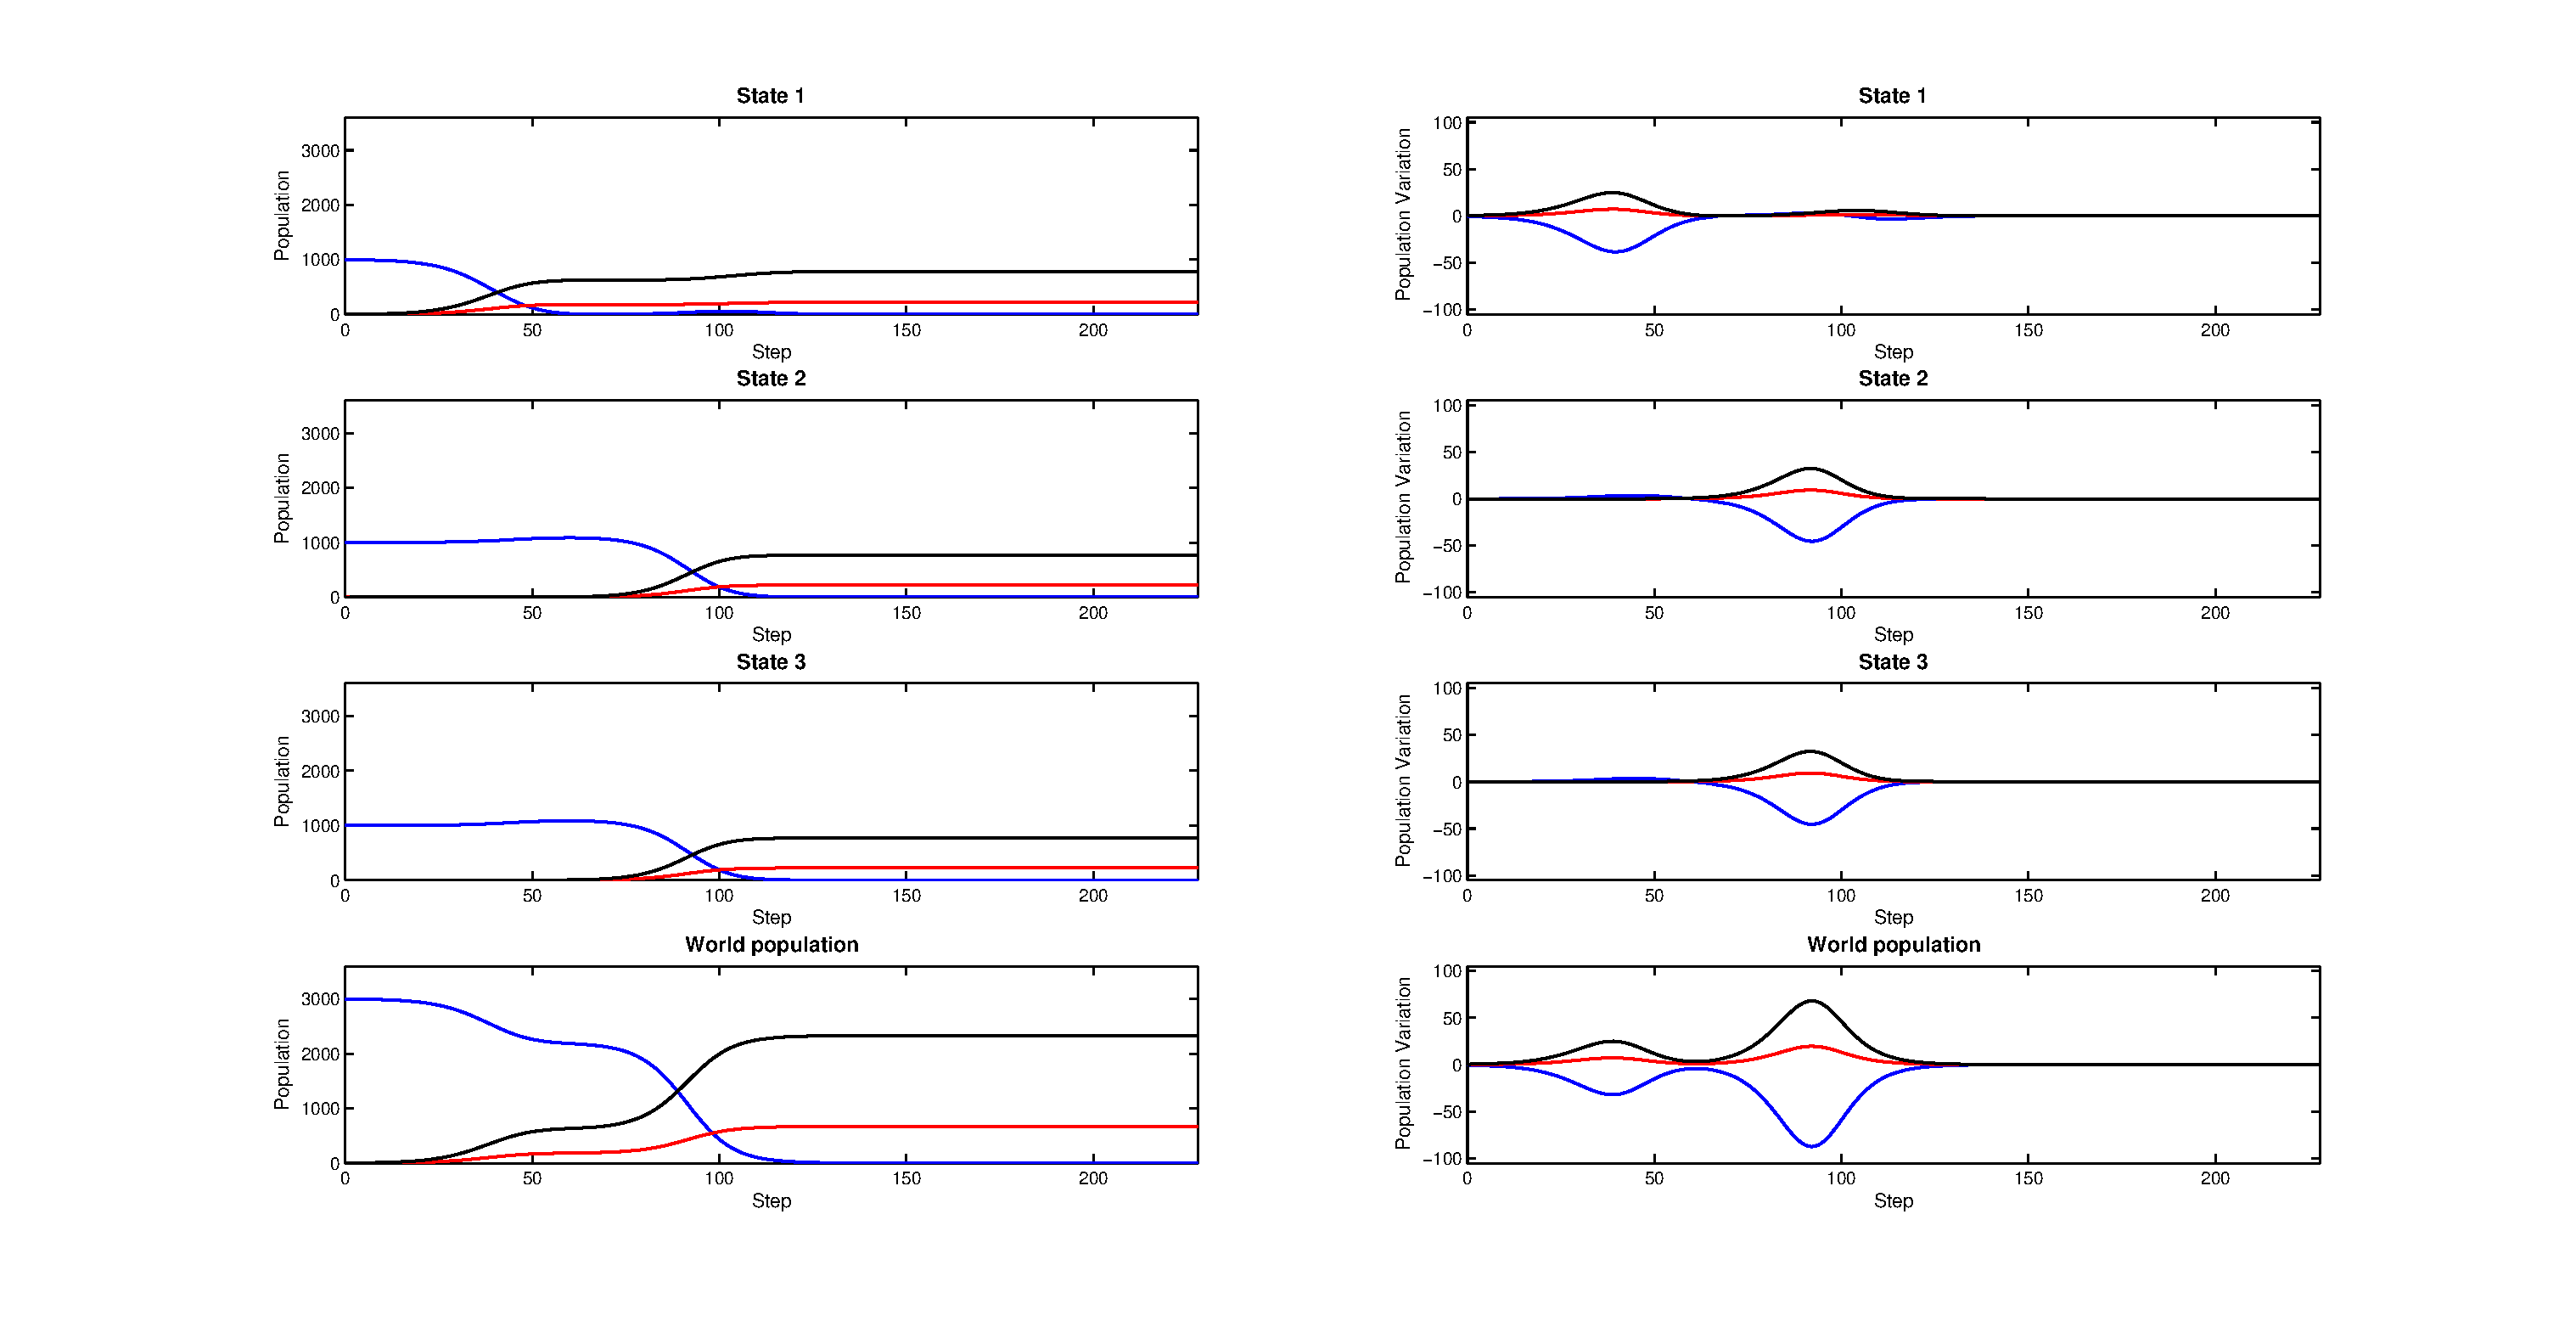
\includegraphics[scale=0.35]{../images/Matlab_figures/example_doomsday.eps}}
\caption{Doomsday scenario. Apparition of a single zombie in state 1 leads to full contamination of the world's population. Left panel represents the populations of each state (and world population) with respect to step number. Right panel represents the corresponding population variation (\textcolor{blue}{blue} = susceptibles, \textcolor{red}{red} = zombies, black = removed, $\alpha=1.5\cdot10^{-4}, \beta=5\cdot10^{-6}, \gamma=5\cdot10^{-4}, \nu=0.1, \eta=1.5\cdot10^{-4}$). \label{doomsday} }
\end{figure}

Interesting observations can already be made by looking at our model under such a regime. In particular, the delayed outbreak in states 2 and 3 due to the necessary accumulation of zombies in state 1 to generate a ratio sufficient to be an incentive for them to migrate to another state with more flesh. This is a direct consequence of our pseudo-flesh-craving model of zombies in their migrational behaviors. Although very weak, we can also observe a small emigration of susceptibles from state 1 to states 2 and 3. Moreover, one can observe that these fluxes are delayed with respect to the death of susceptible in state 1. Again, the explication of this macrostate behavior lies in our description of human migration based on a response to death in their state. The delay originates from the use of a sliding window, which is supposed to represent the lagging-time for people to react and the momentum of large crowd migrations. Overall, we can see that even with the parameter for susceptible migration ($\nu$) larger than the parameter for zombie migration ($\eta$), the escape of susceptible from one state to the other is not sufficient for a survival of the human race. The explanation of it is likely twofold: i) our description of human migration does not properly capture the expected behavior in the event of a zombie outbreak (massive exodus), ii) since $\alpha>\beta$, once a zombie crosses the border, the state is doomed to have its human population eradicated, no matter what and transfer of susceptible cannot change anything to it (see \ref{szr}). 
% Zombie kill figure
\begin{figure}[h!]
\centerline{
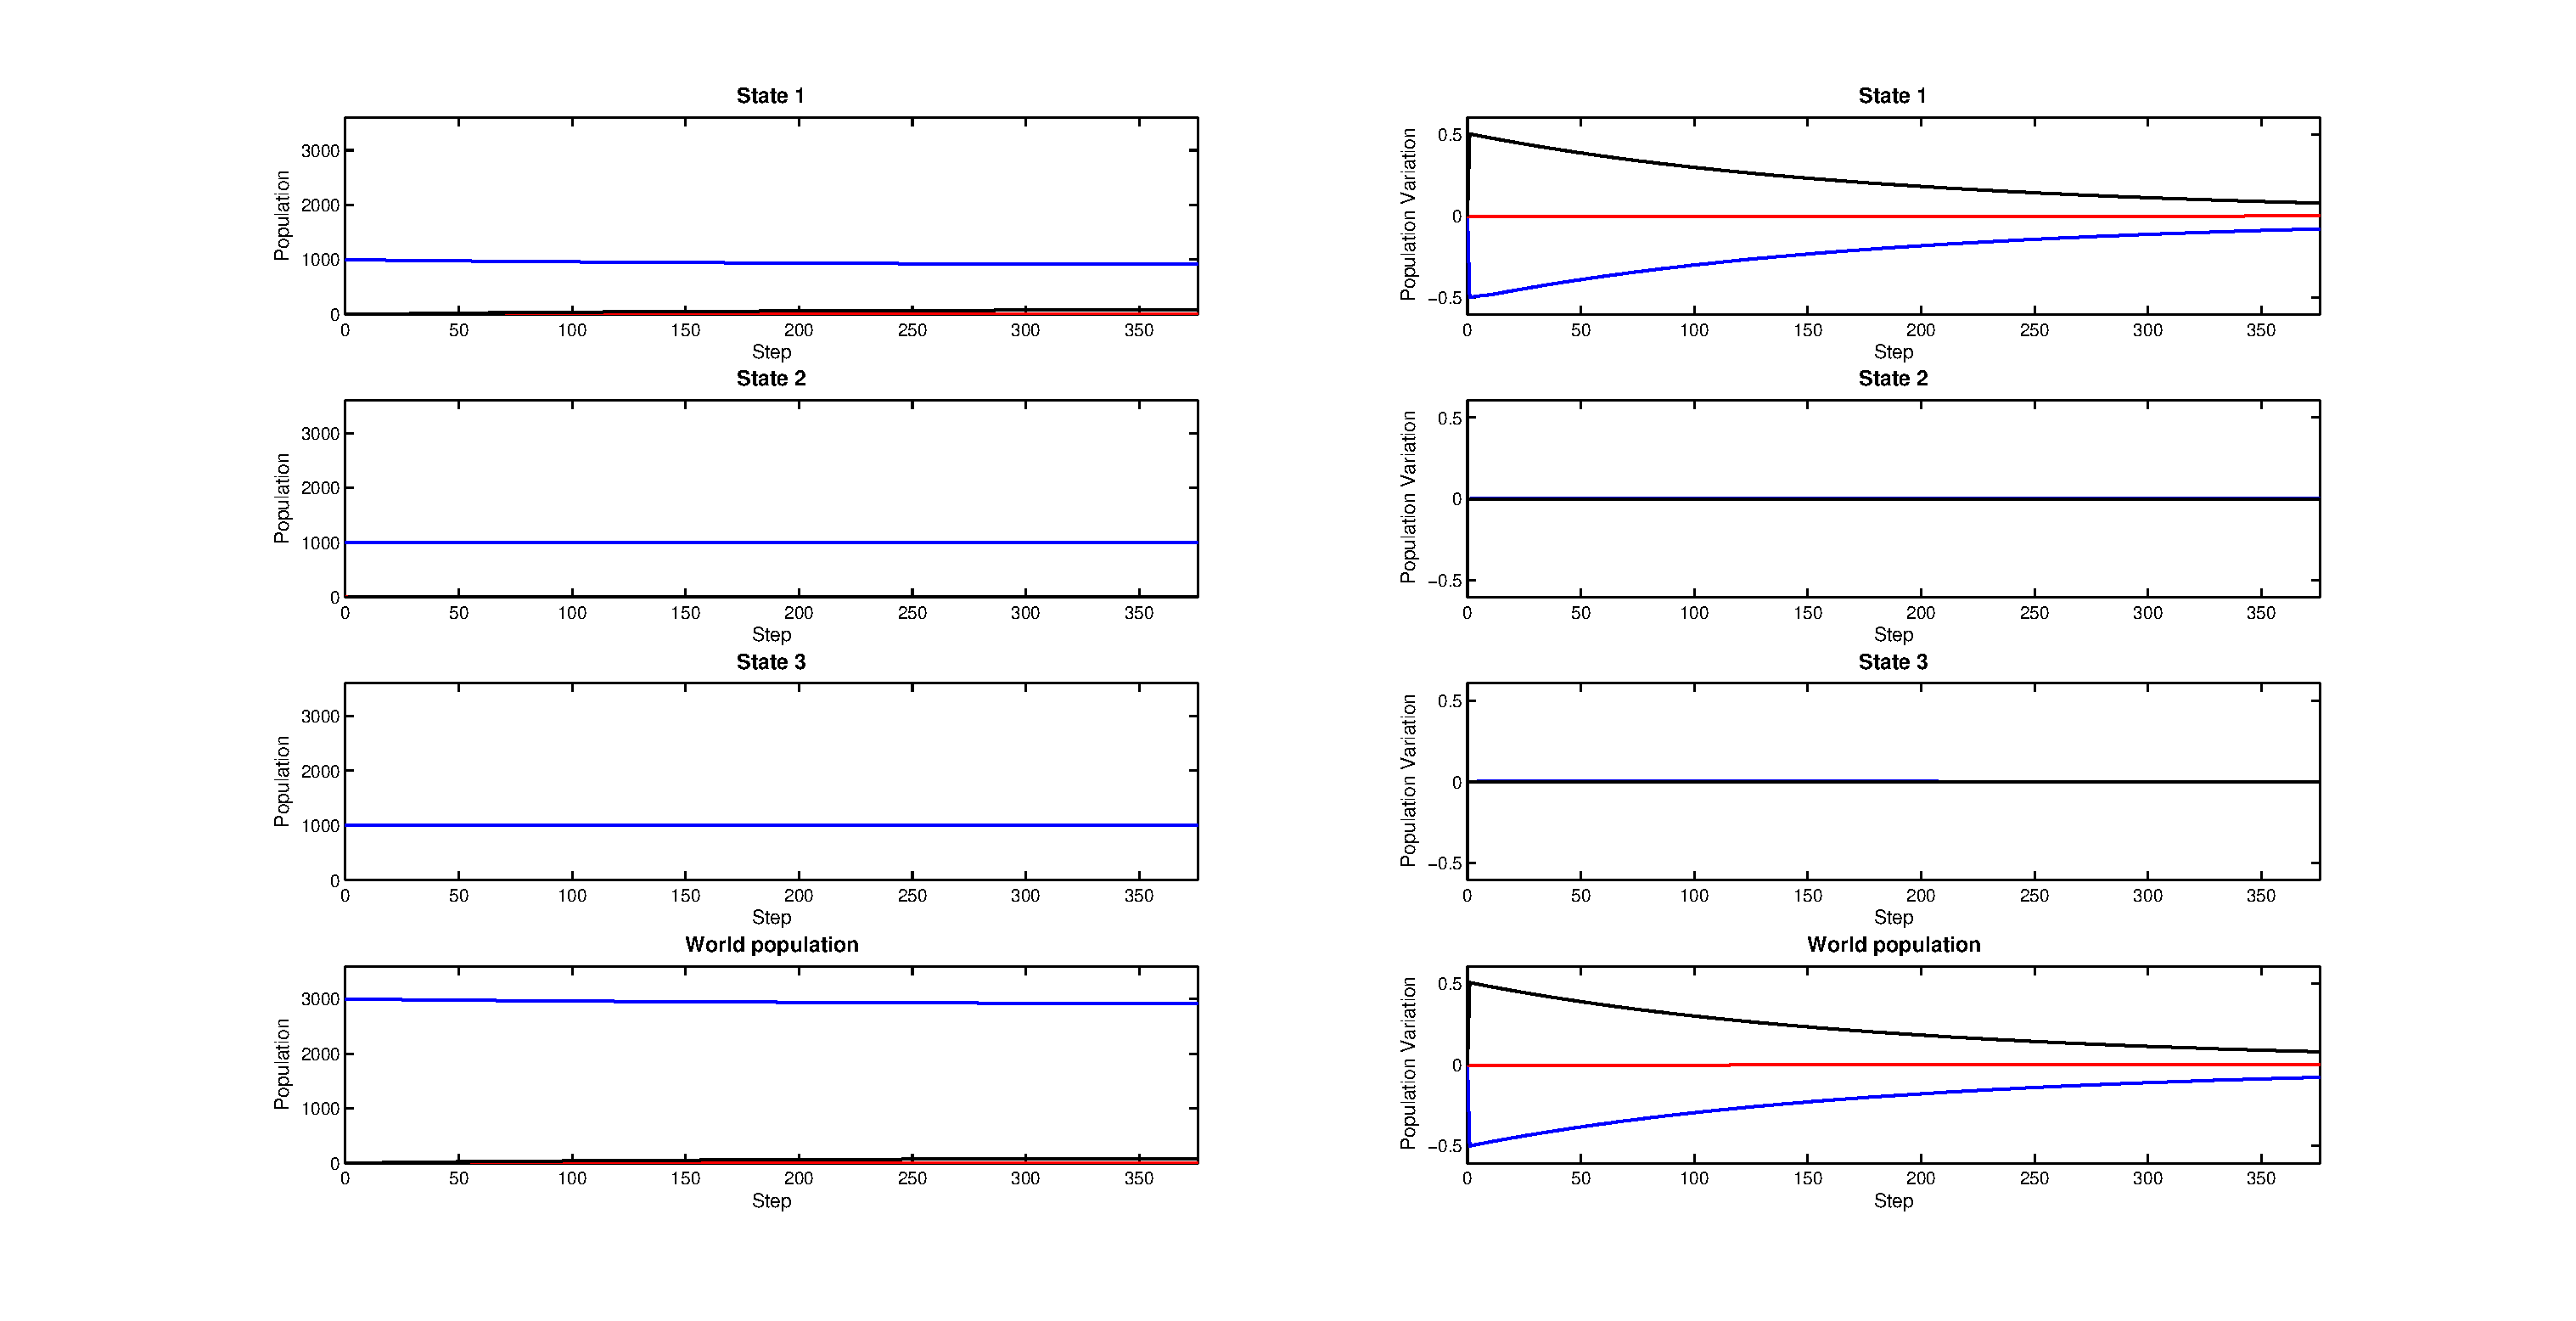
\includegraphics[scale=0.35]{../images/Matlab_figures/example_zkill.eps}}
\caption{Survival of humanity by zombie eradication. As soon as zombies appear in state 1, they get killed until the outbreak is contained. Left panel represents the populations of each state (and world population) with respect to step number. Right panel represents the corresponding population variation (\textcolor{blue}{blue} = susceptibles, \textcolor{red}{red} = zombies, black = removed, $\alpha=1.5\cdot10^{-8}, \beta=5\cdot10^{-6}, \gamma=5\cdot10^{-4}, \nu=0.01, \eta=1.5\cdot10^{-4}$).
\label{skill} }
\end{figure}

A regime where humanity could survive is shown in figure \ref{skill} where it can be seen that emergence of a single zombie in state 1 is not sufficient to generate a burst of the zombie population, due to the $\alpha/\beta$ ratio (see \ref{szr}). This situation is the international analog to what happened in figure \ref{gamma_population}. In such a scenario, the emergence of zombies in state 1 immediately gets crushed, not allowing the build-up of a zombie population that would trigger zombie migration. And even if it would, the fact that zombies get killed more rapidly than they appear would not generate a burst in the other states.




% Exode figure
\begin{figure}[h!]
\centerline{
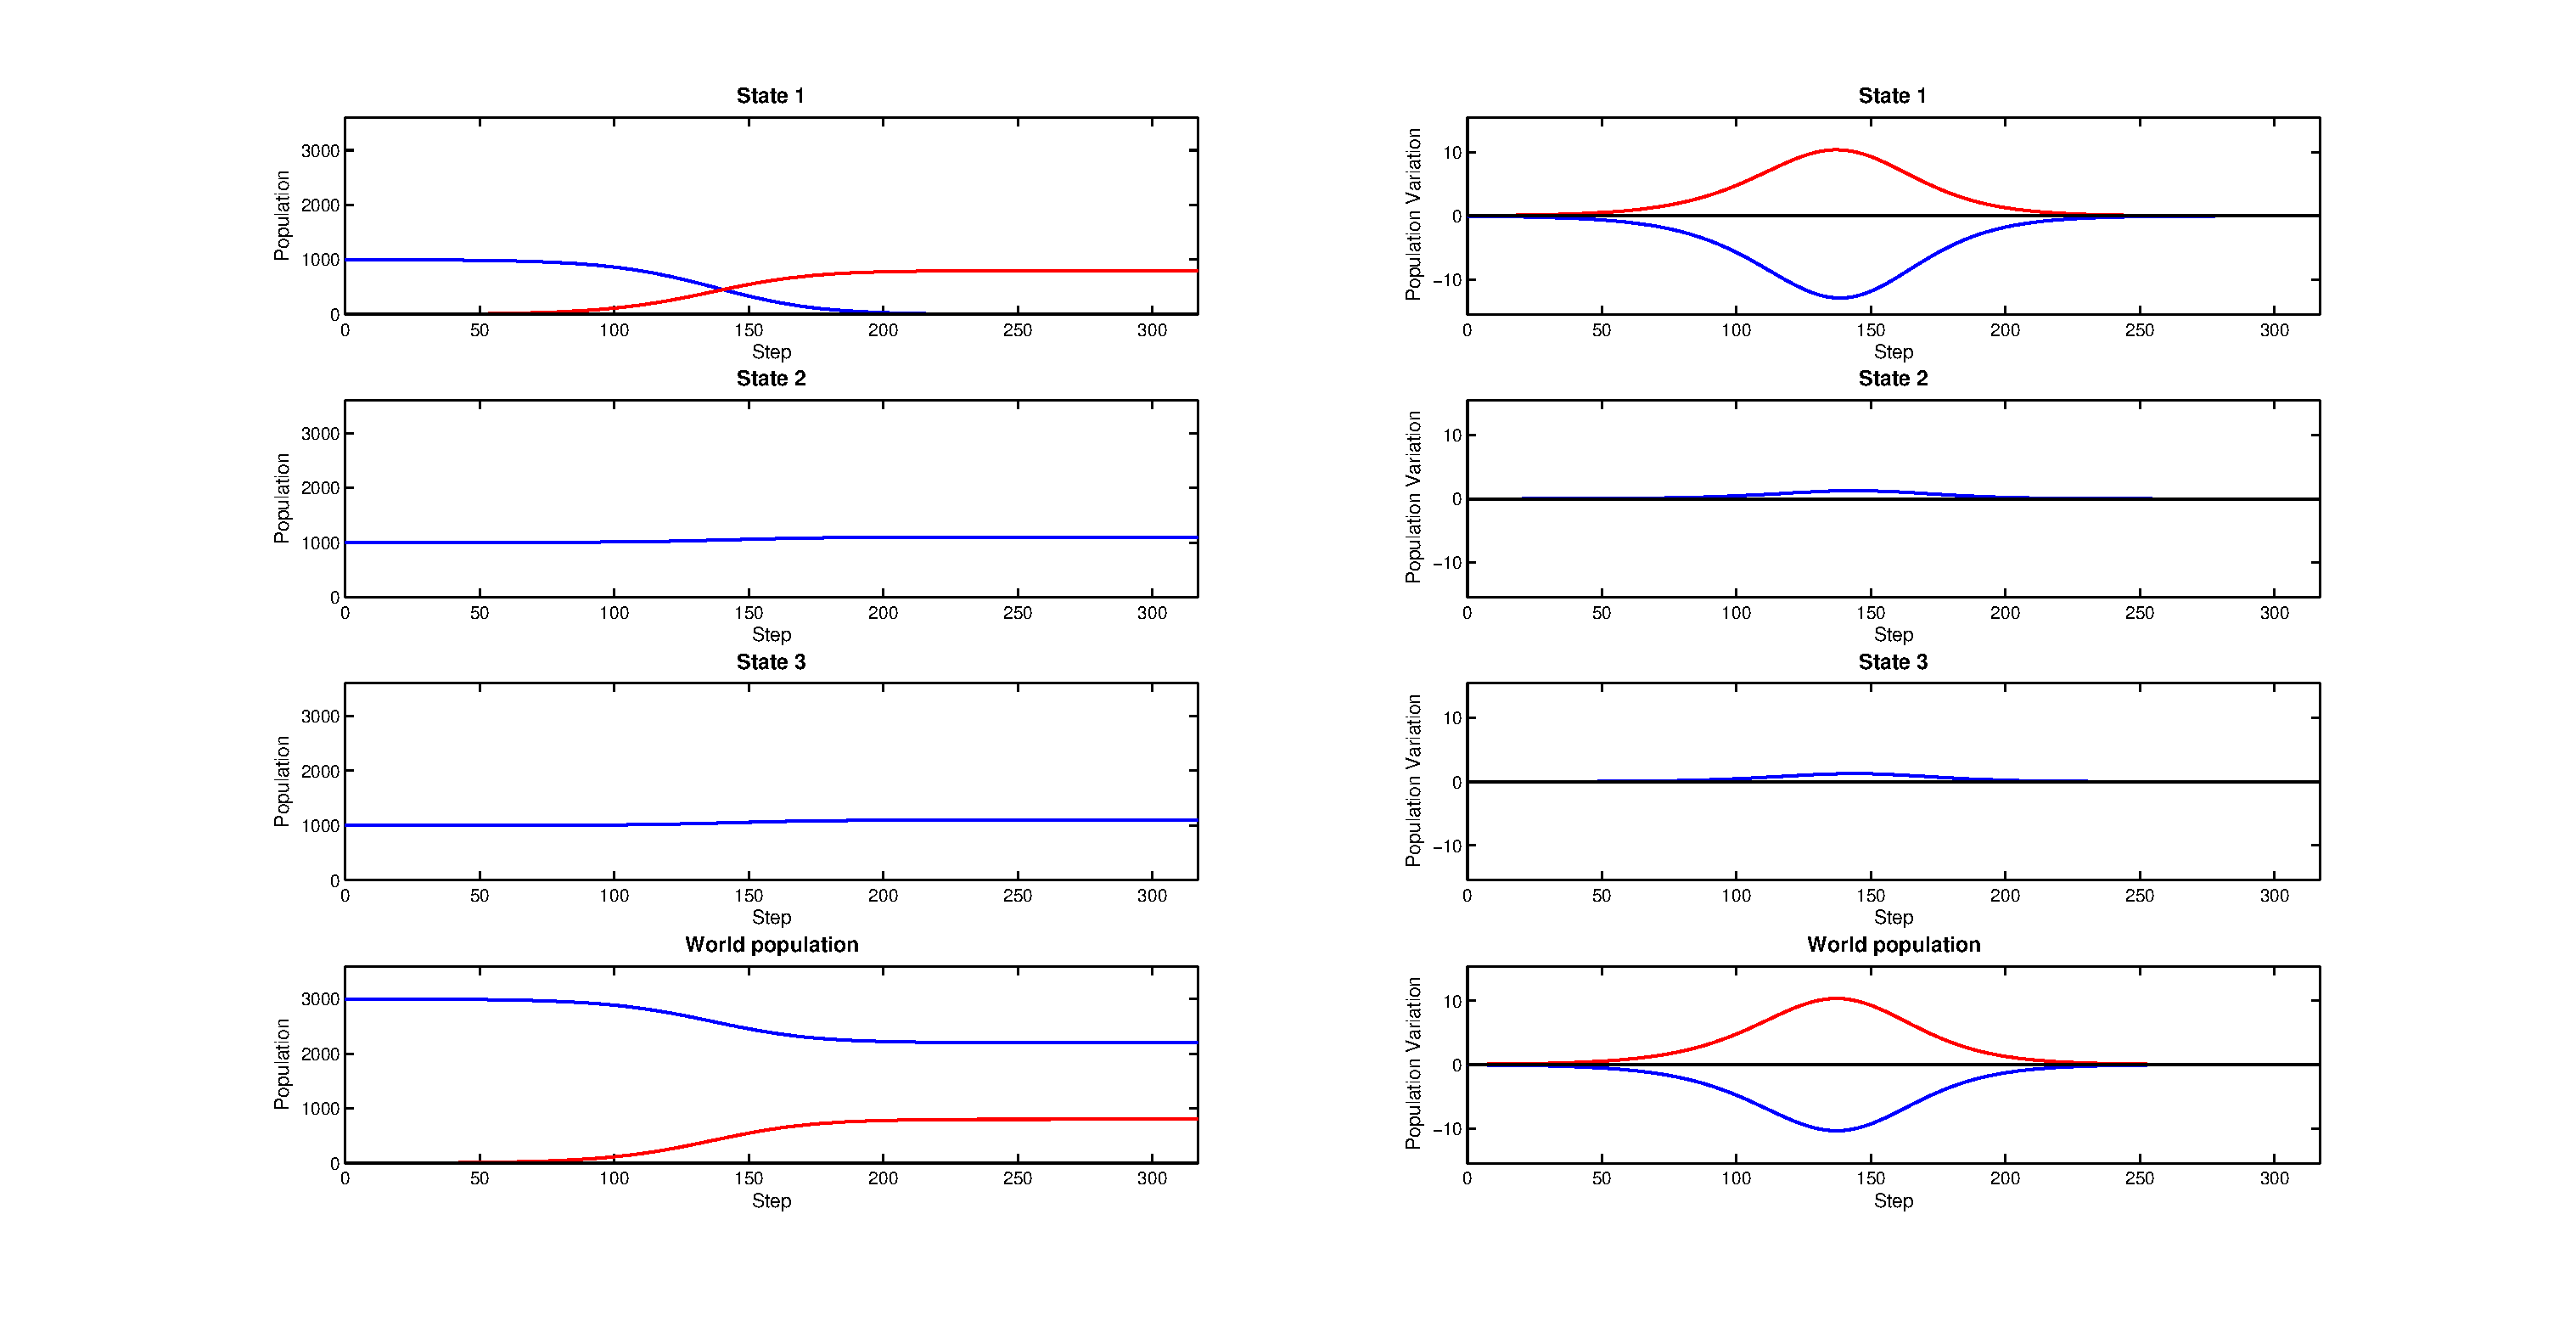
\includegraphics[scale=0.35]{../images/Matlab_figures/example_exode.eps}}
\caption{Survival of humanity and emergence of a zombie state. Emergence of zombies in state 1 leads to the exodus of the remaining population to states 2 and 3. State 1 becomes fully infested with zombies and the remaining of the world's population is in state 2 and 3. Left panel represents the populations of each state (and world population) with respect to step number. Right panel represents the corresponding population variation (\textcolor{blue}{blue} = susceptibles, \textcolor{red}{red} = zombies, black = removed, $\alpha=5\cdot10^{-5},  \beta=5\cdot10^{-10},  \gamma=5\cdot10^{-10},  \nu=0.1,  \eta=0$). \label{exodus} }
\end{figure}

Another example where humanity survives but for a different reason is depicted in figure \ref{exodus}.
Here the set of parameters under scrutiny leads to an interesting phenomenon. Since $\eta=0$ and $\nu$ is large, emergence of a single zombie in state 1 triggers the outbreak and the apparition of a zombie population. Consequently, humans start to feel the urge to move to another place, which they eventually do. The shift in the S to Z ratio should trigger emigration of zombies, but since the borders are closed to for them ($\eta=0$) they can not infest the other states. As a consequence, all remaining susceptibles from state 1 migrate to the other states and the initial location of the outbreak becomes a zombie-only state. Such a scenario can be viewed as a special case of quarantine where an entire country would become depleted from its human inhabitants to the profit of a new population; zombies. Interestingly, this outcome scenario had been postulated by D.W. Drezner for a zombie outbreak in a liberal world order \cite{drezner}. 

\subsection{Phase Transitions for the Micro- and Macro-State Parameters}\indent

So far we treated specific set of parameters, which displayed interesting outcomes corresponding to various scenarios. The next question was to understand the inter-dependence of the parameters with one another in order observe the phase transitions and locations of the interesting regimes of our model. As mentioned before, a complete parameter sweep would not have been feasible due to the number of inter-connected parameters present in our system. Accordingly, we rationalized that since we deconvoluted the behavioral treatment of the micro- and macro-states, we could do the same with the parameter sweep. We first swept $\alpha$, $\beta$ and $\gamma$ under three sets of $\eta$ and $\nu$ to see the phase transitions at the microstate level. We then took a point in this phase-space that presented interesting properties to perform a parameter sweep of $\nu$ and $\eta$. The idea was to find sets of microstate parameters located at phase-transitions and then see how modifying the macrostate parameters could shift the outcome of simulations, \textit{i.e.} how modifying foreign policies could save humanity or lead to its doom.
% 3D plots for alpha beta gamma
\begin{figure}[h!]
\centerline{
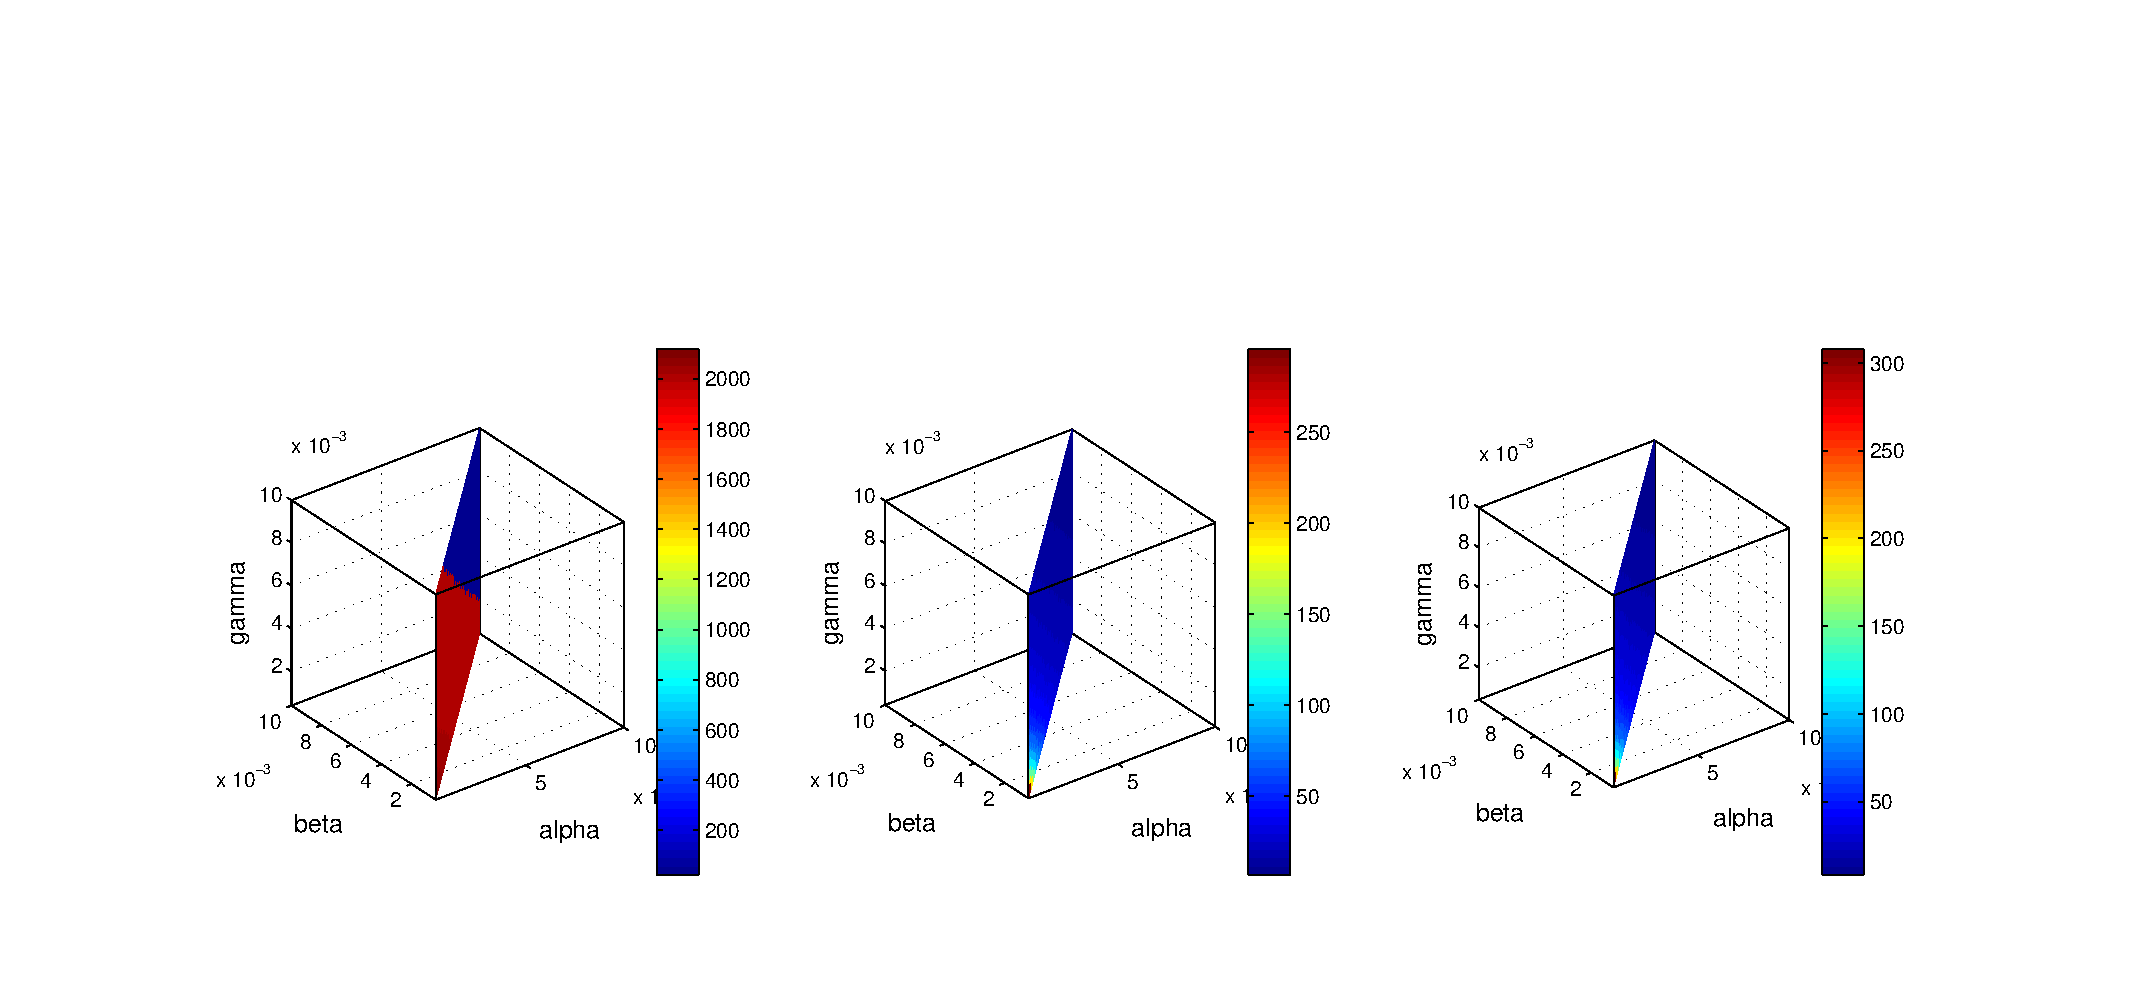
\includegraphics[scale=0.45]{../images/Matlab_figures/a-b-g-sweep.eps}}
\caption{Parameter sweeps for $\alpha$, $\beta$ and $\gamma$ under different $\nu$ and $\eta$. Plotted surface represent the phase-transition between simulations with survivors and simulations with none. The color bar represents the number of humans who survived in each case.  \label{a-b-g} }
\end{figure}

Figure \ref{a-b-g} shows the parameter sweeps for $\alpha$, $\beta$ and $\gamma$ with different sets of $\eta$ and $\nu$. The surface plotted represents the simulations that had a final human population different from zero at the end but a neighbor in the matrix for which it was the case (see \ref{sec:findTransition} for details). Hence, those surfaces represent the transition for sets of $[\alpha, \beta, \gamma]$ between regions of the phase-space where humanity did not survive and regions where it did. In all three cases we can observe a linear relationship between the effect of $\alpha$ and $\beta$ (median plan through the 3D matrix), while the effect of $\gamma$ is negligible. The fact that the choice of different sets of $\nu$ and $\eta$ did not influence the position of the phase-transition validates our approach of separating the micro- and macro-state treatments. It also points out to a small effect of the macrostate parameters on the simulation outcome. The sharp color transition for the left graph of figure \ref{a-b-g} is likely due to an artifact of our implementation and not a physically meaningful result. Indeed, we implemented a termination of the simulation for case where S and Z mean population fluctuation became lower than a threshold (see \ref{outbreakimpl}). It is likely that changing the value of $\gamma$ in this region of the phase-space can switch between an artificially interrupted simulation due to low fluctuation to simulations that end by convergence. 

% Heat map of eta nu sweep
\begin{figure}[h!]
\centerline{
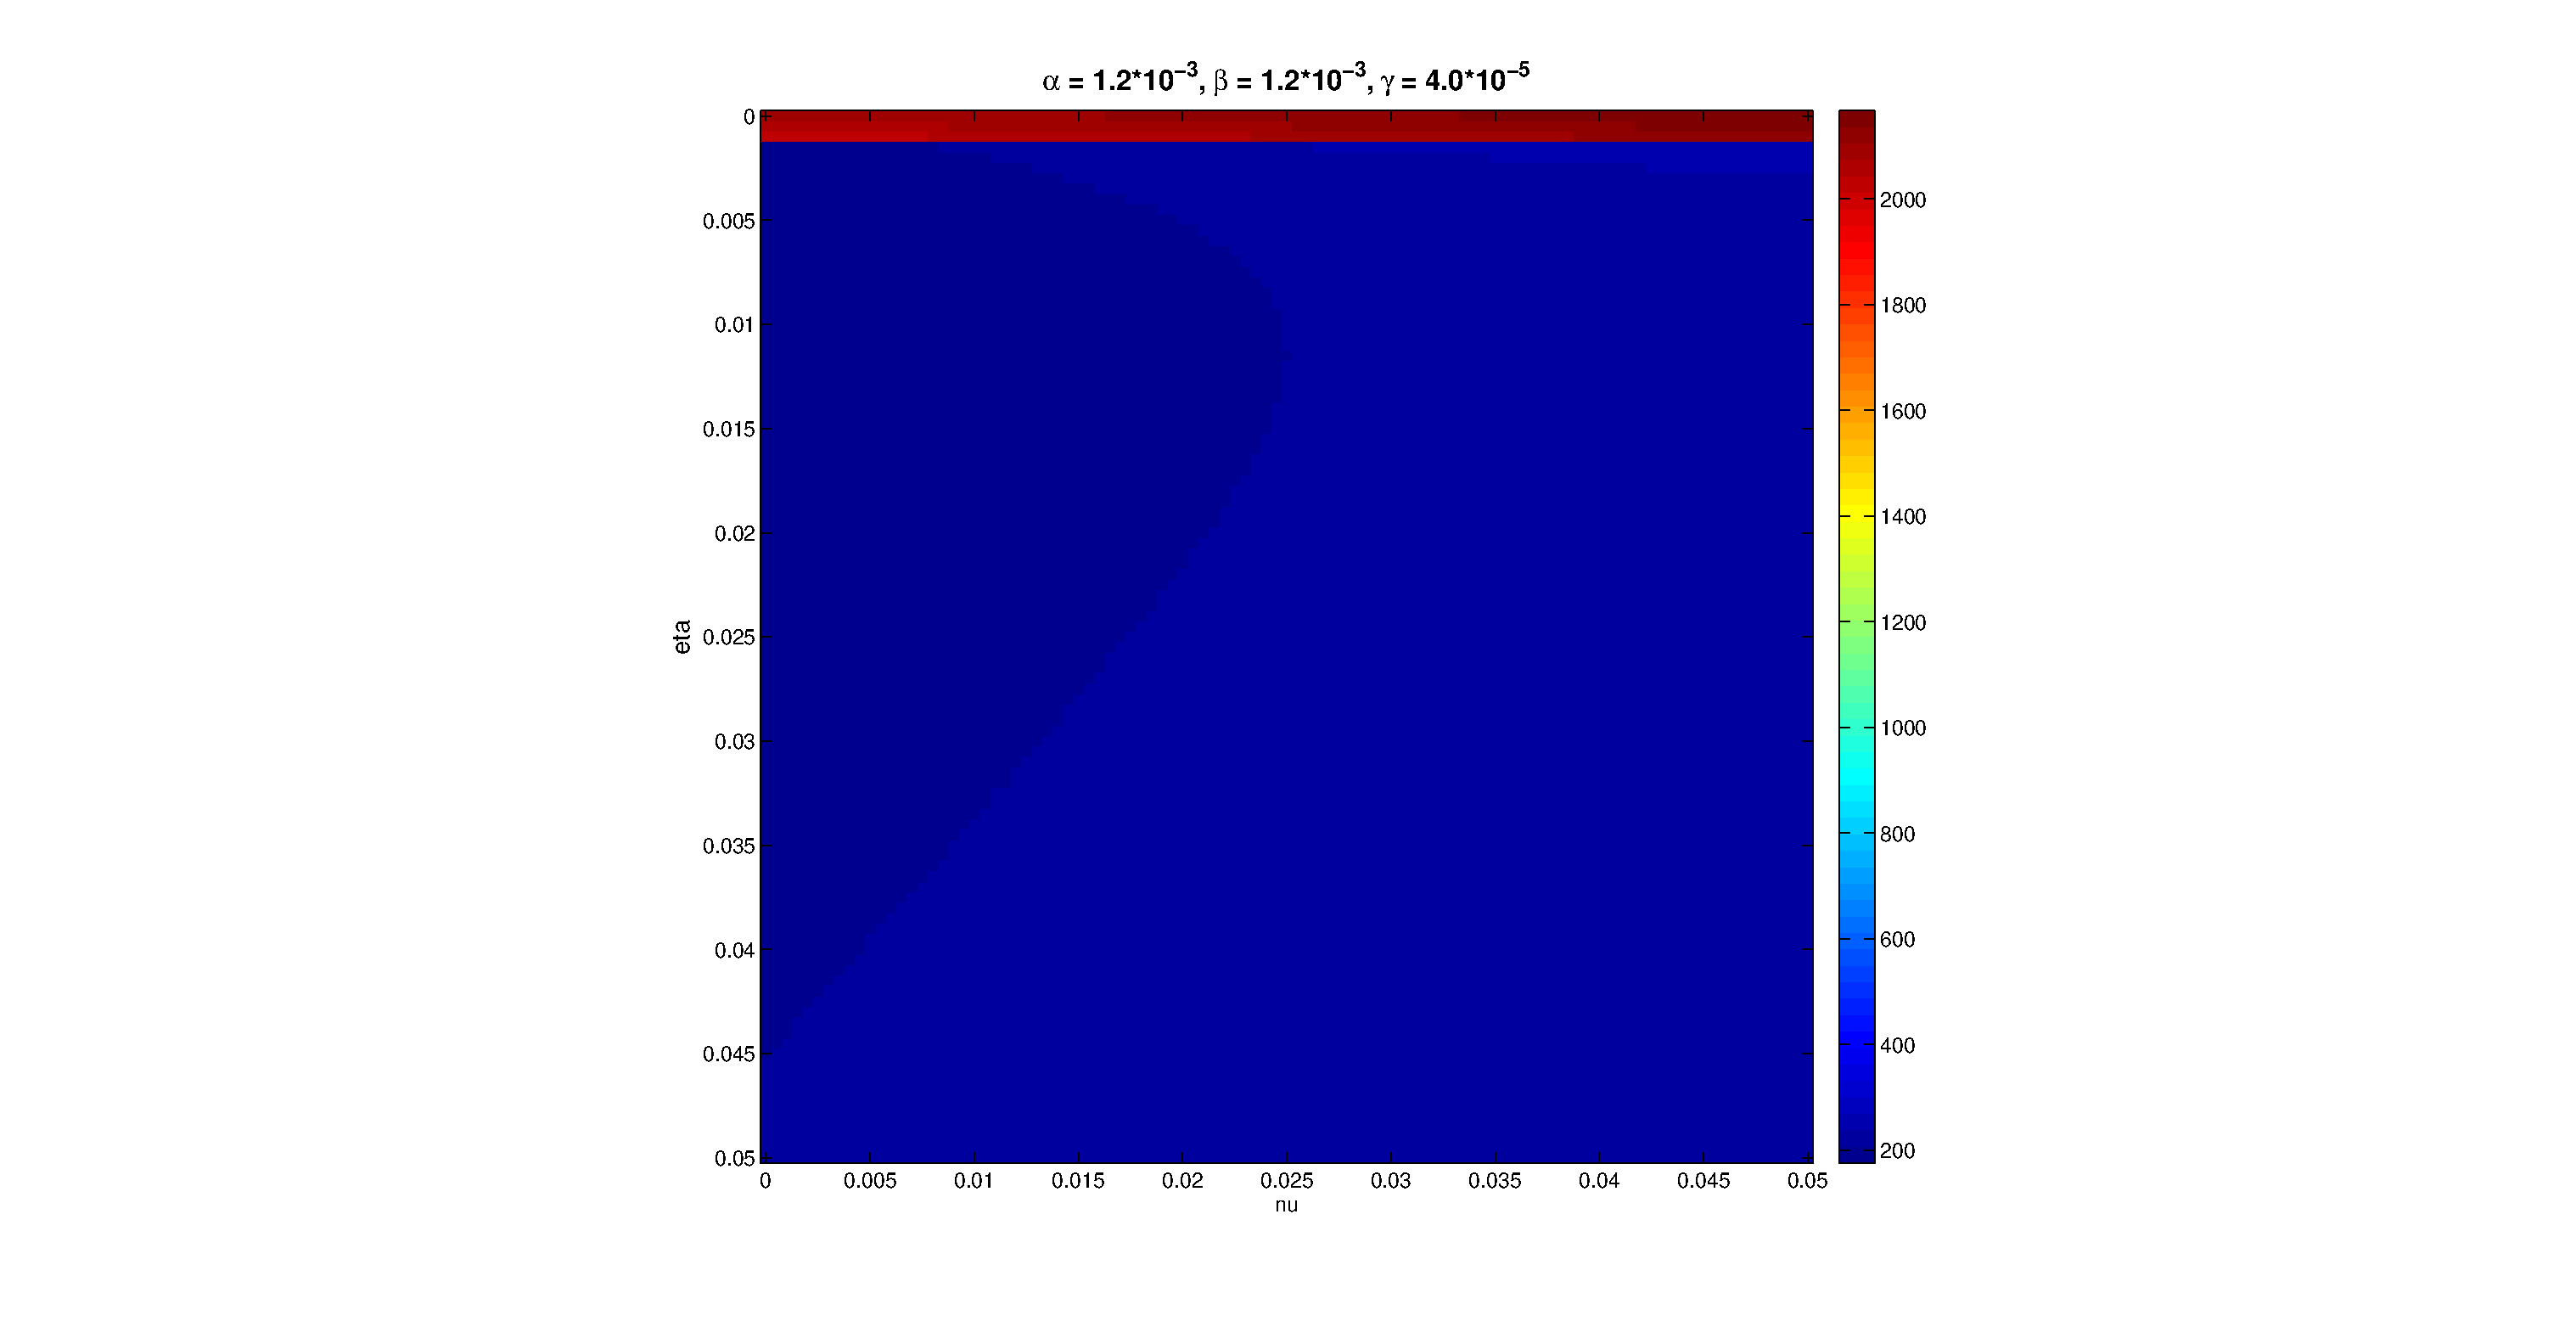
\includegraphics[scale=0.33]{../images/Matlab_figures/nu-eta-sweep.eps}}
\caption{Parameter sweep for $\nu$ and $\eta$ under a fixed  $[\alpha, \beta, \gamma]$ triplet. The color bar represents the number of humans who survived.  \label{nueta} }
\end{figure}


We then decided to chose a point on this transition-surface and use the corresponding $[\alpha, \beta, \gamma]$ triplet to sweep parameters $\nu$ and $\eta$ and observe the phase-transition at the macrostate level. Figure \ref{nueta} shows the heat-map for this parameter sweep. It is worth noting that the upper band of the heat-map that represent a high number of survivors is not really a phase-transition but more a limit of our model with the parameters under consideration. Indeed, it represents the case were the transfer of zombies is zero or almost inexistent, making the contamination of the other state impossible (hence the high number of survivors). For the rest of the phase-diagram, we observe a biphasic system. The reason for this behavior is unclear, in particular the absence of a real gradient but it might be due to the threshold value used to stop the simulation when fluctuations become small. Nevertheless, it can pointed out that increasing $\eta$ (transfer of zombies) lowers the number of survivors, consistent with our intuition. However, a more interesting result is the less favorable outcome when $\nu$ (transfer of susceptibles) is increased to large values. One might think about this result as counter-intuitive since transferring more humans to non-contaminated states should help. But macrostate transfers should be considered in both directions, meaning that in the case $\nu$ and $\eta$ large, susceptibles will start fleeing the zombie outbreak, but since the zombies will then follow, humans will try to go back to their initial states. This back-and-forth pattern of human migration can be deleterious to the general outcome when its magnitude becomes to large, hence explaining the phase transition when increasing $\nu$.



\subsection{Asymmetric State Powers}\indent
\label{sec:asym}

So far we have only looked at fully symmetrical systems where both populations and parameters under scrutiny were chosen equal for every state. We did so in order to avoid introduction of additional effects on the simulation outcomes, which would have been hard to deconvolute from the rest of the features of our model. Another reason was that certain parameters simply represent ``physical constants'' of zombification, \textit{i.e.} they are independent of the state under consideration and are only related to the zombie outbreak paradigm under consideration. Parameters that fall into this category are typically $\alpha$ and $\gamma$. Indeed, it is likely that zombification will occur at the same rate everywhere since it is an epidemiological parameter and should therefore not be influenced by factors such as socio-economical environments. Under the assumptions of our model, the same consideration hold for $\gamma$. Parameters $\nu$ and $\eta$ could arguably be different between states but for the sake of simplicity, we decided to model cooperation in systems of homogenous international relationships. Finally, $\beta$, which represent the efficiency of the people in a given state to kill zombies, was so far set as identical in all systems for symmetrical reasons. However, a more accurate representation of the international scene implies considering a world containing states possessing different military powers. 

\begin{figure}[h!]
\centerline{
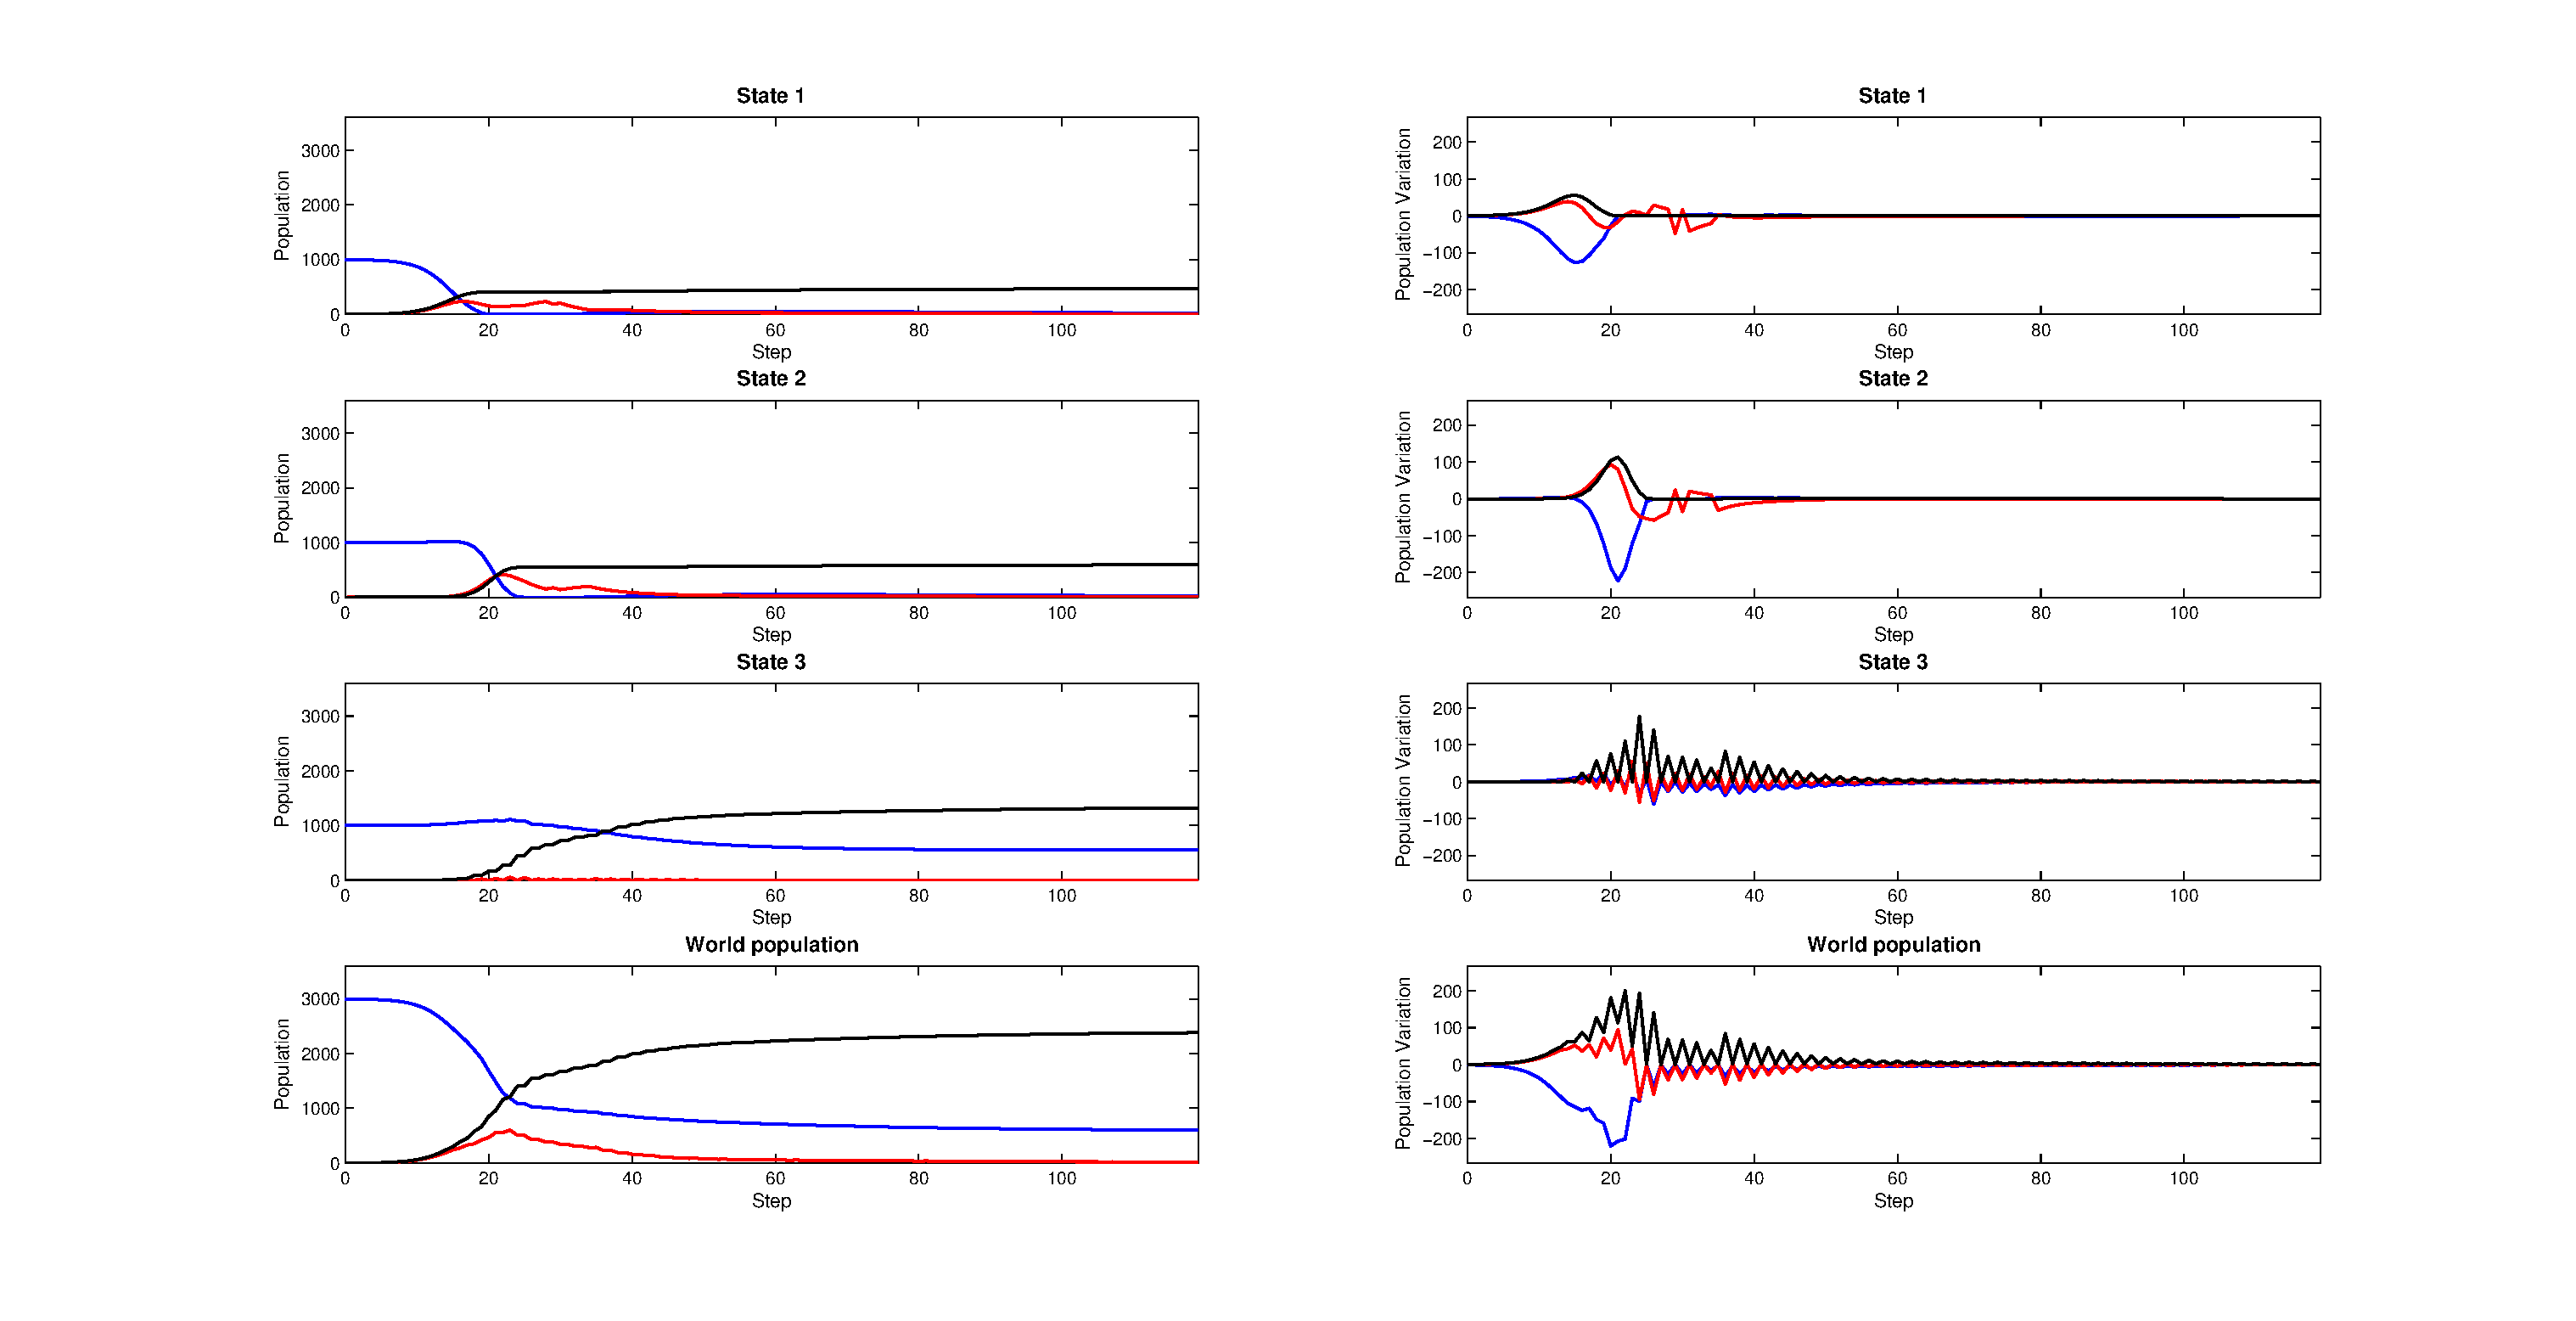
\includegraphics[scale=0.35]{../images/Matlab_figures/asymmetric-system.eps}}
\caption{The effect of asymmetry in state powers.  Emergence of zombies in state 1 leads to contamination and partial death in states 1 and 2, leading to the emigration of both susceptibles and zombies to the other states.  State 3 possessing a higher $\beta$ value, the outbreak is crushed at the border, leading to zombie eradication. Left panel represents the populations in each state (and world population) with respect to step number. Right panel represents the corresponding population variation (\textcolor{blue}{blue} = susceptibles, \textcolor{red}{red} = zombies, black = removed, $\alpha=1.0\cdot10^{-3}, \beta=5\cdot10^{-4} $ (states 1 and 2) $\beta=5\cdot10^{-3}$ (state 3) $, \gamma=1\cdot10^{-4}, \nu=0.25, \eta=0.1$). \label{basym} }
\end{figure}


A simple way to represent such an effect within the framework of our model would simply be to assign different $\beta$ to the three states. Figure \ref{basym} represents such a case, where state 3 possesses a value for $\beta$ larger than states 1 and 2. Such a system displays interesting features. First of all, it is worth noting that since $\alpha>\beta$ in state 1, a zombie outbreak occurs, leading to contamination and death of the susceptibles in that state. A similar effect is observable for state 2 for the same reason, however with a delay (accumulation of zombies in state 1 before they start emigrating). Those features are consistent with the observations made in section \ref{sec:time-evolv} and figure \ref{doomsday}. Indeed, $\alpha$ being greater than $\beta$, zombies appear with a rate higher than their eradication, leading to disappearance of humans in those states. Emigration of susceptible is also observable after the zombie outbreak. But most interestingly, it can be observed that the higher value of $\beta$ in state 3 (with $\beta>\alpha$ unlike state 1 and 2) allows to avoid a zombie outbreak in this particular state. Moreover, and contrary to the case observed in figure \ref{exodus}, apparition of a zombie state does not occur. Indeed, once state 1 and 2 are depleted from their populations of susceptibles, zombies start emigrating to state 3 where they immediately get killed at the border, eventually leading to global eradication of all the zombies. This behavior provides an interesting modeling of a case where an outbreak would lead to people fleeing and finding refuge in another state where the fate of humanity would be decided in a total war against zombies until none remain.





% SUMMARY AND OUTLOOK
\newpage
\section{Summary and Outlook}\indent

In the present study we showed the behavior of interconnected SZR models as a way to represent international cooperation in the event of a zombie outbreak. We investigated the role of the inter-state migration fluxes in relation to the survival of humanity. Due to the lack of empirical precedents, it has been challenging to define a model that could grasp the complexity of such a scenario. In particular, we encountered problems in the modeling of the macrostate level fluxes due to the high interconnectivity of the equations, which led to implementation difficulties. The model described here treats the population evolution at the microstate level within an epidemiological framework, while the macrostate level is described with a reaction-based migration of susceptible (with inertia) and a pseudo-flesh-craving paradigm for the transfer of zombies. Due to the lack of data that could have allowed us to generate the parameters needed for our description, we performed a parameter sweep to find the phase transitions of our model. The high dimensionality of our system raised further challenges that we tackled by treating the parameter sweep of the micro- and macro-state independently. 

Owing to the symmetry of the systems investigated, location of the phase-transitions were fairly straightforward. Furthermore, it seemed that within our description, the microstate behavior dominated the outcome. We were able to find limit cases where our model displayed interesting behaviors. In particular, the standard doomsday scenario with zombie overcoming the world (and attempt of the susceptible to migrate with no effect) as well as the emergence of a zombie state in the case where borders would not let any zombies cross. Finally, presence of asymmetry in the description of state powers revealed that full eradication of zombies was possible to the cost of emptying the weaker state from their populations. In conclusion, we can postulate that in order to give humanity its best chances, international policies should quickly adapt to let all humans immigrate to state that are not yet contaminated and very firmly watch their borders for zombies.
  
\subsection{Further Investigations: Asymmetric systems}\indent

In section \ref{sec:asym} we described the effect of an asymmetric $\beta$ value on the global outcome. This proved to yield an interesting scenario for the survival of humanity within the framework of our model. One could imagine varying the other parameters of our system to see the effect on the simulation outcomes. In particular, asymmetric population sizes could be interesting to study, as well as attributing different macrostate parameters ($\nu$ and $\eta$) to the states. Finally, changing the initial number of zombies or introducing zombie outbreaks in multiple subpopulations could give interesting regimes, although unlikely to be favorable to the survival of humanity.

\subsection{Further Investigations: Game-Theoretical Treatment of Inter-State fluxes}\indent
\label{sec:gt}

For each state (microstate), a SZR evaluates the evolution of the different populations under study. Mass-action transfer of populations between the states (at the macrostate level, \textit{i.e.} international level) also occurs as defined in our model and simulates refugee and zombie transfers across states. Those transfers are dependent of parameter $\nu$ for susceptible transfer and parameter $\eta$ for zombie transfer. Within the scope of this semester project, we decided to simulate different regimes of international cooperation by simply fixing the values of $\eta$ and $\nu$ at the beginning of each simulation and observe the resulting outcomes. Both the relative and absolute values of those parameters are supposed to represent the paradigm of international politics under consideration (\textit{e.g.} a very small value of $\nu$ would represent neo-conservatism since it drastically limits the possibility of refugee immigration). Of course, such a treatment is very static and does not take into account the likely variation over time of international cooperation elements (change in immigration policies, military action on foreign soil, etc...); a variation likely to occur when dealing with a zombie outbreak.

Therefore, a elegant way to make the macrostate parameters ($\nu$, $\eta$) dynamic and allow the representation of such changes would be to make them functions of a game-theoretical treatment. Similar approaches for other epidemiological studies have been described in the literature as a way to provide a more realistic approach to disease spreading in human populations \cite{funk2010modelling, reluga2010game, reluga2009sis}. In such a system, population fluxes would still be treated within the framework of our current model, with the only variation that the macrostate parameters would be time-evolving. 

\bigskip

\textit{Microstate treatment} $\Rightarrow$ \textit{SZR model} 

\bigskip

\textit{Macrostate treatment} $\Rightarrow$  $\left\{
	\begin{array}{l l}
		\Delta S_{i}^{macro} =  \sum_{j\neq i}{ \left( \textcolor{red}{\nu} \langle \Delta S_{j} \rangle - \textcolor{red}{\nu}  \langle \Delta S_{i} \rangle \right) }	
    \\
    \\
    		\Delta Z_{i}^{macro} = \sum_{j\neq i}{\left( \textcolor{blue}{\eta} Z_{j}\tanh \left( \frac{Z_{j}}{S_{j}}\right) -\textcolor{blue}{\eta} Z_{i}\tanh \left( \frac{Z_{i}}{S_{i}}\right) \right)}

	\end{array} \right.$

\bigskip

\textit{where} \textcolor{red}{$\nu$} $= f(GT)$ \textit{,} \textcolor{blue}{$\eta$} $= f(GT)$  
\bigskip


Changing the values of $\nu$ and $\eta$ over the course of the simulation would be under cost-hypothesis as defined in game-theory and the cost-hypothesis themselves would become fixed parameters, thus defining the different paradigms of international politics. The apparition of zombies in one state would start the game. Each state would then evolve on the domestic and international levels. The domestic level would follow the standard SZR model, whereas the international level would introduce exchanges of populations between the states. These exchanges will be influenced by the state's decisions in foreign policies. Modifying $\nu$ and $\eta$ would be defined with a specific payoff, which in turn will depend on the international cooperation system under scrutiny. For simplicity, models should be treated homogeneously, \textit{i.e.} all states should adopt the same international politics paradigm. Finally, a ``feedback'' loop on the payoff, depending on the success of a previously undertaken action (positive or negative affectation of the payoffs), could be introduced. This effect could be a way to model the psychological effect of a successful or unsuccessful past action on future undertakings, for example the effectiveness of a military attack. The system would be implemented as a step-based update, implying the actor's (the states) ignorance of the other actor's actions. This rationalization would be consistent with the idea of an outbreak occurring over a short period of time, forcing rapid decision-making and therefore not allowing a reaction-based decision-making process. 





% REFERENCES
\newpage

\bibliography{zombie_report} % Load the .bib file containing the references
\bibliographystyle{unsrt} % Define bibliography style
%\nocite{bennett1995modelling, balcan2011phase, funk2010modelling, reluga2010game, reluga2009sis}



% APPENDIX
\newpage

\section{Appendix}
\bigskip
\subsection{outbreak.m}
\label{sec:outbreak}
\lstinputlisting{../code/outbreak.m}
\bigskip
\bigskip
\bigskip

\subsection{update.m}
\label{sec:update}
\lstinputlisting{../code/update.m}
\bigskip
\bigskip
\bigskip

\subsection{sweep.m}
\label{sec:sweep}
\lstinputlisting{../code/sweep.m}
\bigskip
\bigskip
\bigskip

\subsection{findTransition.m}
\label{sec:findtrans}
\lstinputlisting{../code/findTransition.m}





\end{document}  



 
